\documentclass[11pt,a4paper,oneside]{report}
\usepackage[utf8]{inputenc}
\usepackage[T1]{fontenc}
\usepackage{lmodern}
\usepackage[provide=*,italian]{babel}
\usepackage[a4paper,left=25mm,right=23mm,top=24mm,bottom=25mm,headheight=15pt]{geometry}
\usepackage{microtype,graphicx,xcolor,booktabs,tabularx,longtable,array,amsmath}
\usepackage{enumitem,titlesec,fancyhdr,caption,float,tikz}
\usetikzlibrary{arrows.meta,positioning,calc,fit,shapes.geometric}
\usepackage[numbers,sort&compress]{natbib}
\usepackage{xurl,hyperref}
\definecolor{PortaleInk}{HTML}{173C44}
\definecolor{PortaleAccent}{HTML}{A2613B}
\definecolor{PortalePale}{HTML}{EDF2F1}
\hypersetup{colorlinks=true,linkcolor=PortaleInk,citecolor=PortaleInk,urlcolor=PortaleInk,pdftitle={Il Portale: una infrastruttura civica per imparare musica},pdfauthor={Fabrizio Terzi},pdfsubject={Monografia tecnica di progetto v0.5}}
\titleformat{\chapter}[display]{\normalfont\color{PortaleInk}}{\sffamily\small IL PORTALE\quad /\quad\chaptertitlename\ \thechapter}{8pt}{\Huge\bfseries\raggedright}
\titlespacing*{\chapter}{0pt}{0pt}{24pt}
\titleformat{\section}{\Large\bfseries\color{PortaleInk}}{\thesection}{0.7em}{}
\titleformat{\subsection}{\large\bfseries}{\thesubsection}{0.7em}{}
\setcounter{secnumdepth}{2}
\setcounter{tocdepth}{1}
\setlength{\parskip}{4pt}
\setlength{\parindent}{0pt}
\setlength{\emergencystretch}{3em}
\setlist[itemize,enumerate]{nosep,leftmargin=*,topsep=6pt}
\setlist[description]{style=unboxed,leftmargin=0pt,labelindent=0pt,labelwidth=0pt,labelsep=0.6em,font=\bfseries,topsep=6pt,itemsep=5pt}
\captionsetup{font=small,labelfont=bf}
\pagestyle{fancy}\fancyhf{}
\fancyhead[L]{\small\sffamily IL PORTALE}
\fancyhead[R]{\small\sffamily Ricerca e progetto / v0.5}
\fancyfoot[R]{\thepage}
\renewcommand{\headrulewidth}{0.3pt}
\fancypagestyle{plain}{\fancyhf{}\fancyfoot[R]{\thepage}\renewcommand{\headrulewidth}{0pt}}
\newcolumntype{P}[1]{>{\raggedright\arraybackslash}p{#1}}
\newcolumntype{Y}{>{\raggedright\arraybackslash}X}
\newcommand{\projectnote}[1]{\begin{quote}\small\color{PortaleInk}#1\end{quote}}
\begin{document}
\begin{titlepage}
\color{PortaleInk}
{\sffamily\small PYRAGOGY / PEERAGOGIA\hfill RICERCA DI PROGETTO}\par
\vspace{15mm}
{\fontsize{44}{48}\selectfont\bfseries Il Portale}\par
\vspace{5mm}
{\LARGE Una infrastruttura civica\\per imparare musica}\par
\vspace{5mm}
{\large Forma, interazione, apprendimento tra pari\\e vita pubblica a Parco Caprotti}\par
\vspace{9mm}
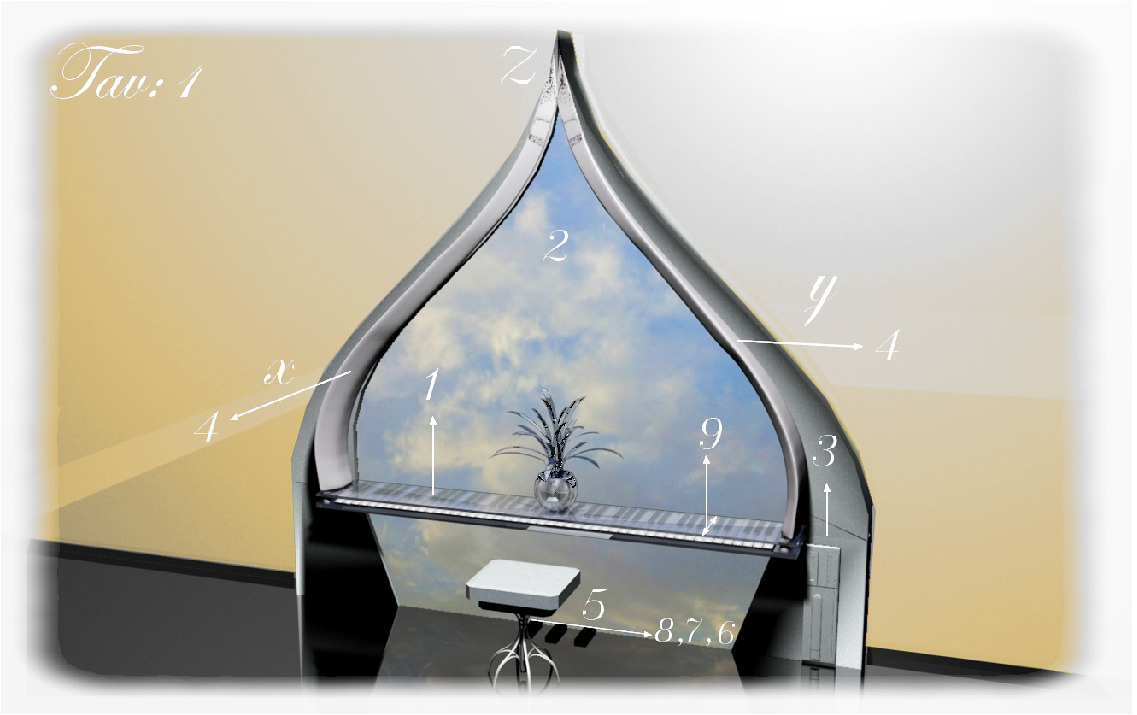
\includegraphics[width=\linewidth]{figures/portale-originale-2016.jpg}\par
\vspace{5mm}
{\small Il disegno originale: un luogo raccolto attorno al gesto musicale.\\Documento di Fabrizio Terzi, 2016, p.\ 3; immagine inalterata.}\par
\vfill
{\large Fabrizio Terzi}\par
\vspace{3mm}
{\sffamily Monografia tecnica v0.5 / 18 ottobre 2026}\par
{\small Dal concept documentato 2013--2016 a una proposta verificabile.\\Edizione per revisione critica: progetto, specifiche e protocollo di prova.}
\end{titlepage}
\pagenumbering{roman}
\chapter*{Tesi e statuto del documento}
\addcontentsline{toc}{chapter}{Tesi e statuto del documento}
Il Portale propone di rendere l'apprendimento musicale una possibilità ordinaria dello spazio pubblico: un luogo riconoscibile in cui il gesto individuale possa diventare ascolto reciproco, esplorazione e conoscenza condivisa. La forma a goccia raccoglie tastiera, immagine e suono; il programma educativo e la gestione civica devono trasformare questa presenza in una pratica durevole.

La tesi di questa monografia è che il valore del progetto vada cercato nella qualità delle relazioni fra cinque elementi: forma abitabile, risposta musicale immediata, possibilità di apprendere tra pari, risorse riutilizzabili e responsabilità pubblica della cura. Nessuno di questi elementi, isolatamente, prova un primato. La loro integrazione costituisce il contributo progettuale da mettere alla prova.

Il documento sviluppa una proposta di sistema, ne confronta gli antecedenti, specifica requisiti, alternative, prove e condizioni di sostenibilità. Parco Caprotti è indicato nel documento originale; il Padiglione del Tè è una candidatura contemporanea da discutere con chi ne regola e anima gli usi. Non sono qui presentati un'installazione realizzata, un accordo con gli enti, risultati sperimentali o una certificazione tecnica.

\textbf{Come leggere le affermazioni.} I fatti documentali hanno una fonte citata. Le scelte progettuali definiscono una configurazione proposta. Le soglie numeriche e i budget sono assunzioni da sottoporre a collaudo o a preventivo, salvo esplicita indicazione contraria. Le ipotesi educative e civiche richiedono dati futuri. Una simulazione geometrica rende discutibile una soluzione; non ne dimostra acustica, sicurezza o efficacia.

\textbf{Responsabilità editoriale.} Il concept e la direzione del progetto sono di Fabrizio Terzi. Questa edizione è stata redatta con assistenza ChatGPT e sei agenti specialistici, con integrazione e revisione interna. Pi ha revisionato la precedente v0.3; la sua approvazione non viene estesa automaticamente a questo testo. Il protocollo allegato consente una nuova revisione indipendente e un confronto fra redazioni LLM. Non è stata svolta una peer review scientifica esterna della v0.5.

\tableofcontents
\clearpage\pagenumbering{arabic}
\chapter{Una possibilità musicale nella vita della città}\label{ch:thesis}

\section{Il diritto di cominciare}
Una città offre molte occasioni per consumare musica e occasioni assai più diseguali per farla. Si può ascoltare ovunque; per provare a suonare occorrono invece uno strumento, un luogo, un tempo consentito e, spesso, la sensazione di essere già abbastanza capaci. Il Portale nasce attorno a questa soglia. Il suo primo compito è rendere possibile un inizio: sedersi, produrre un suono, sentirne una risposta, riconoscere che il gesto successivo dipende da noi.

Questa è una posizione di progetto. Non descrive un bisogno già misurato tra i frequentatori di Parco Caprotti: quella ricerca va condotta. Definisce però un problema abbastanza preciso da orientare forma, tecnologia e programmazione. Se la postazione attraesse soltanto chi sa già suonare, avremmo forse un buon strumento pubblico, ma non avremmo ancora verificato la sua promessa educativa. Se offrisse un'interazione spettacolare senza lasciare alcuna scelta musicale alla persona, avremmo indebolito il nucleo stesso dell'idea.

Il gesto iniziale contiene una questione civica: chi si sente autorizzato a occupare lo spazio con la propria presenza e con il proprio suono? Una tastiera pubblica può rendere visibile questa possibilità. Può anche produrre esitazione, esposizione e conflitto. Per questo il Portale deve offrire più modi di partecipare: osservare, ascoltare, provare in raccoglimento, affiancare un'altra persona, proporre una variazione. La libertà di entrare nell'esperienza comprende quella di non esibirsi.

L'ambizione è costruire un piccolo luogo nel quale la città possa ascoltarsi mentre impara. Il valore non risiede soltanto nell'oggetto che vi si posa: risiede nella relazione che l'oggetto rende praticabile e nella disponibilità a custodirla nel tempo.

\section{Che cosa contiene davvero il documento originale}
Il documento conservato nel repository reca la data del 1 gennaio 2016 e, nella descrizione del modello, la dicitura interna \emph{Filed: Gen.\ 20, 2013}. Questi sono elementi documentali, non prove autonome di deposito legale, priorità brevettuale o pubblicazione scientifica. La fonte presenta la struttura a goccia, l'interazione audiovisiva, la tastiera MIDI, la pedaliera, l'unità di calcolo, risorse musicali online e tutoraggio; prevede inoltre una webcam e la trasformazione durante l'inattività in mensola e galleria di immagini. La scheda finale nomina il \emph{Learning City Point} e localizza la proposta nel parco comunale dei Caprotti, via Tasso, Bergamo \cite[pp.~2--5]{terzi_peeragogy_2016}.

È già presente una concatenazione di intenzioni: un oggetto compatto rende disponibile la pratica; lo schermo mette in relazione il gesto con altri materiali; la rete apre il luogo a risorse e persone lontane; la trasformazione a riposo mantiene una presenza architettonica; il riferimento al parco colloca l'apprendimento dentro la città. La lettura contemporanea deve sviluppare queste relazioni, esplicitando quali sopravvivono e quali richiedono una nuova decisione.

La fonte include formulazioni tecniche da riesaminare, fra cui il riferimento a \emph{Dolby Stereo Spectral Recording} e diverse tecnologie di schermo. Qui non diventano requisiti da riprodurre letteralmente. La configurazione proposta partirà dalla qualità dell'ascolto, dalla leggibilità e dalla manutenzione. Il marketplace di tutoraggio menzionato nella fonte apre inoltre una questione economica distinta dall'accesso civico gratuito al nucleo della postazione. La nuova proposta conserva la possibilità di incontri con tutor, ma non assume che un servizio commerciale sia necessario all'esperienza iniziale.

\section{La bellezza come relazione progettata}
La forma a goccia ha una forza che una semplice lista di dispositivi non restituisce. Disegna un contorno attorno all'esecutore e rende riconoscibile l'incontro fra corpo, tastiera e immagine. Non possiamo dedurne automaticamente comfort o qualità acustica; possiamo però riconoscere una precisa scelta compositiva. La tecnologia viene raccolta in una figura che invita a essere avvicinata e che resta presente quando l'attività si interrompe.

La bellezza del progetto dipende dalla coerenza fra questa promessa visiva e ciò che una persona riesce effettivamente a fare. Una struttura che suggerisce accoglienza deve permettere di entrare e uscire con agio. Un'immagine che invita a esplorare deve lasciare iniziativa. Una postazione che dichiara condivisione deve offrire posto anche a chi ascolta o aiuta. Un oggetto destinato al giardino deve sapere convivere con il silenzio. Queste relazioni diventano criteri di progetto, osservabili e discutibili.

\section{Dall'oggetto al sistema civico}
La monografia assume tre scale collegate. La prima è il gesto: risposta dello strumento, leggibilità, postura, controllo. La seconda è la relazione: alternanza, ascolto, facilitazione, materiali condivisi. La terza è la città: accesso, compatibilità degli usi, gestione, risorse e memoria delle attività. Il fallimento a una scala può annullare il lavoro svolto alle altre. Una latenza disturbante impedisce il dialogo musicale; un presidio assente può rendere inutilizzabile un oggetto ben costruito; una programmazione esclusiva può allontanare proprio le persone a cui era rivolto.

\begin{figure}[htbp]
\centering
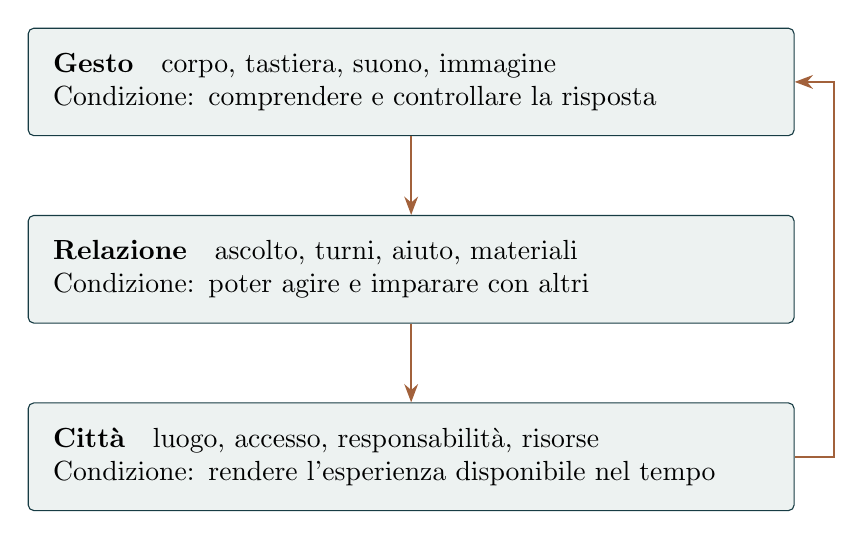
\begin{tikzpicture}[node distance=10mm,box/.style={draw=PortaleInk,rounded corners=2pt,fill=PortalePale,text width=0.75\linewidth,align=left,inner sep=9pt},arr/.style={-{Stealth},thick,PortaleAccent}]
\node[box] (g) {\textbf{Gesto}\quad corpo, tastiera, suono, immagine\\Condizione: comprendere e controllare la risposta};
\node[box,below=of g] (r) {\textbf{Relazione}\quad ascolto, turni, aiuto, materiali\\Condizione: poter agire e imparare con altri};
\node[box,below=of r] (c) {\textbf{Città}\quad luogo, accesso, responsabilità, risorse\\Condizione: rendere l'esperienza disponibile nel tempo};
\draw[arr] (g)--(r);\draw[arr] (r)--(c);
\draw[arr] (c.east) -- ++(0.5,0) |- (g.east);
\end{tikzpicture}
\caption{Tre scale del progetto. Le condizioni di gestione tornano a determinare ciò che il singolo gesto può offrire: il sistema deve essere verificato lungo l'intera relazione. Schema progettuale, non risultato empirico.}
\end{figure}


\chapter{L'originalità come relazione: uno strumento, un luogo, una comunità}
\label{sec:originality}

La domanda decisiva per Il Portale è quale possibilità venga aggiunta alla vita della città. Una tastiera pubblica offre accesso a uno strumento. Uno schermo mette a disposizione contenuti. Un collegamento permette di incontrare qualcuno lontano. Il progetto diventa interessante quando queste possibilità cambiano reciprocamente funzione: lo strumento invita a fermarsi, l'immagine rende comprensibile un gesto, un'altra persona offre una risposta, il luogo rende possibile ritrovarsi. L'oggetto acquista allora un compito ambizioso: dare una forma materiale al passaggio fra il desiderio di fare musica e la possibilità di impararla insieme.

Questa è la tesi progettuale che proponiamo di sottoporre a prova. La sua originalità va argomentata attraverso antecedenti, scelte e conseguenze osservabili. Il documento del 2016 testimonia una formulazione del concept e ne contiene i disegni; le diciture relative a inventore e deposito presenti nella fonte non sono qui assunte come certificazione di brevetto, priorità legale o realizzazione materiale \cite[pp.~2--5]{terzi_peeragogy_2016}. Il confronto seguente è una ricognizione mirata, non una ricerca esaustiva di anteriorità. Serve a individuare ciò che il progetto eredita e ciò di cui deve dimostrare il valore.

\section{Tre antecedenti che cambiano il problema}

\paragraph{Il pianoforte pubblico: rendere legittimo l'incontro.}
\emph{Play Me, I'm Yours}, ideato da Luke Jerram, fu commissionato a Birmingham nel 2008, con quindici pianoforti disponibili in luoghi della città. Nella ricostruzione dell'autore, la motivazione nasce dall'osservazione di persone che condividono un luogo senza parlarsi; lo strumento deve offrire un'occasione di relazione \cite{conc_streetpianos}. Questo antecedente impedisce di attribuire al Portale l'invenzione dell'accesso musicale spontaneo nello spazio pubblico. Offre invece una domanda esigente: quale esperienza aggiuntiva giustifica la complessità di computer, schermo, materiali didattici e gestione dei contenuti? La risposta proposta riguarda il passaggio dall'esecuzione all'apprendimento condiviso. Dovrà essere verificata anche con persone che, davanti a uno strumento disponibile, non si sentono ancora autorizzate a provarlo.

\paragraph{Reactable: rendere leggibile l'azione musicale.}
Il gruppo della Universitat Pompeu Fabra avviò Reactable nel 2003 e ne presentò una prima esecuzione pubblica nel 2005. Lo strumento impiega una superficie tangibile sulla quale gli oggetti e le loro relazioni controllano processi sonori; il lavoro del 2007 discute l'incontro fra performance musicale e interfacce da tavolo \cite{conc_reactable,conc_jorda2007}. La relazione fra gesto, visualizzazione e musica, così come la possibilità di costruire strumenti digitali collaborativi, ha dunque antecedenti precisi. Per Il Portale ne deriva una responsabilità: definire che cosa lo schermo renda intelligibile. Mostrare colori che reagiscono al suono può essere una scelta estetica legittima; per sostenere un'ipotesi didattica occorre indicare quale relazione musicale la persona possa riconoscere, riprodurre o modificare grazie a quella rappresentazione.

\paragraph{La città che apprende: mantenere una possibilità nel tempo.}
La cornice UNESCO delle learning cities include l'accesso all'apprendimento negli spazi pubblici, la partecipazione degli attori locali, la valutazione e la sostenibilità delle risorse \cite{conc_learningcity}. Il nome \emph{Learning City Point}, presente nel documento originale, viene qui utilizzato come denominazione del progetto, senza attribuirgli uno status UNESCO. Il riferimento è utile per una ragione concreta: una postazione diventa un'opportunità educativa urbana quando qualcuno se ne assume la cura, quando le attività sono raggiungibili e quando esistono percorsi per proseguirle. La connessione di rete, da sola, non produce nessuna di queste condizioni.

\section{Il contributo proposto e il suo termine di paragone}

Il contributo che vale la pena sviluppare consiste nell'organizzare quattro continuità: fra osservare e provare; fra il proprio gesto e la risposta di un'altra persona; fra un incontro breve e una pratica successiva; fra la memoria di un luogo e la possibilità di produrvi nuova cultura. Queste continuità attraversano livelli diversi del sistema. La prima riguarda l'interfaccia e la disposizione nello spazio; la seconda le attività e la facilitazione; la terza i materiali e le occasioni di ritorno; la quarta il rapporto con chi vive e cura il luogo. La loro integrazione è una proposta progettuale. Non è ancora un risultato sperimentale.

\begin{table}[htbp]
\centering
\small
\begin{tabular}{P{0.19\linewidth}P{0.33\linewidth}P{0.37\linewidth}}
\hline
\textbf{Riferimento} & \textbf{Possibilità documentata} & \textbf{Questione per Il Portale} \\
\hline
Pianoforte pubblico & Accesso allo strumento e occasione d'incontro nello spazio urbano. & Quale sostegno permette anche a un principiante di iniziare e tornare? \\
Reactable & Interazione musicale tangibile e visualizzazione delle relazioni fra controlli. & Quali rappresentazioni aiutano a capire e trasformare il proprio gesto? \\
Learning city & Partecipazione, accessibilità, organizzazione e continuità dell'apprendimento. & Chi garantisce disponibilità, cura e collegamenti con altre opportunità? \\
Il Portale, proposta & Un oggetto riconoscibile collega gesto, risorse e scambio in un luogo civico. & L'integrazione produce benefici sufficienti a giustificarne costi e complessità? \\
\hline
\end{tabular}
\caption{Confronto delle funzioni rilevanti. Le prime tre righe sintetizzano i riferimenti discussi; la quarta descrive un'intenzione da verificare. L'assenza di una funzione nella tabella non dimostra che un antecedente ne sia privo.}
\label{tab:antecedents}
\end{table}

Il termine di paragone deve restare vicino alla scelta reale di una città. Un pianoforte accessibile, accompagnato da un facilitatore e da poche attività ben costruite, potrebbe ottenere risultati migliori di un'installazione sofisticata. Il Portale dovrà quindi essere confrontato anche con questa alternativa credibile. Una valutazione rispetto alla sola assenza di attività confonderebbe il valore dell'iniziativa culturale con quello della specifica architettura. E attribuire al dispositivo gli effetti di una persona particolarmente capace di coinvolgere il pubblico nasconderebbe il vero motore dell'esperienza.

\section{La bellezza concettuale ha conseguenze operative}

La forma a goccia raccoglie nell'originale corpo, tastiera e schermo. Leggiamo questa disposizione come il tentativo di dare consistenza a una soglia: un interno abbastanza riconoscibile da invitare a entrare nell'attività, un'apertura sufficiente a mantenere il rapporto con ciò che accade attorno. È un'interpretazione del disegno, non una qualità ergonomica già misurata. Per trasformarla in progetto occorre verificare visibilità, accesso, spazio laterale, postura e possibilità di affiancamento. Se il secondo partecipante può soltanto osservare alle spalle dell'esecutore, la promessa di cooperazione incontra un limite fisico preciso.

Anche la trasformazione prevista durante l'inattività merita una lettura rigorosa. La tastiera convertibile in mensola e la funzione di galleria audiovisiva suggeriscono un oggetto che mantiene una presenza nel luogo quando nessuno suona. Il comportamento inattivo dovrà rendere percepibile la disponibilità all'uso e distinguere la pausa dal guasto. Un'immagine continua potrebbe invece farlo scambiare per un espositore; un suono dimostrativo potrebbe disturbare chi cerca quiete. La qualità formale si misura anche in questa discrezione: lasciare intuire una possibilità senza pretendere attenzione permanente.

Per una città, la bellezza di tale oggetto può consistere nel rendere visibile una fiducia: anche chi passa senza un titolo musicale può contribuire. Questa è una posizione culturale del progetto. Per darle concretezza servono inviti comprensibili, un primo gesto reversibile, assenza di classifiche pubbliche all'ingresso e il diritto di restare soltanto ad ascoltare. La competenza deve poter emergere senza diventare il prezzo d'accesso. Lo stesso principio richiede profondità: chi sa suonare deve trovare margini espressivi reali e la possibilità di contribuire senza essere ridotto al ruolo permanente di dimostratore.

\section{Progettare anche per chi guarda}

Il lavoro di Reeves e colleghi sull'esperienza dello spettatore mostra come le interfacce pubbliche possano rendere più o meno visibili le azioni di chi le usa e i loro effetti \cite{conc_reeves2005}. Per Il Portale, considerare questa relazione significa progettare un insieme di posizioni: chi esegue, chi osserva, chi attende, chi vorrebbe partecipare. L'osservatore fa parte dell'esperienza anche quando non tocca un comando. La leggibilità del gesto può favorire una domanda; l'esposizione eccessiva può rendere difficile il primo tentativo.

Proponiamo perciò due condizioni dichiarate: esplorazione raccolta e condivisione. Nella prima la persona controlla l'ascolto e può provare senza dover sostenere un pubblico. Nella seconda rende disponibili il suono e, se utile, la rappresentazione dell'attività. Il passaggio deve essere esplicito e reversibile. La precisa soluzione acustica e visiva dipenderà dal sito; qui interessa il requisito: nessuna attività dovrebbe trasformarsi involontariamente in un'esibizione. Analogamente, la presenza di un pubblico non deve impedire a un secondo partecipante di entrare in relazione. Occorrono spazio, turni leggibili e attività con ruoli che possano essere scambiati.

\section{Una memoria musicale costruita nel luogo}

Il carattere locale può emergere dai contributi che l'oggetto rende possibili. Proponiamo una raccolta curata di brevi materiali: una frase da variare, un accompagnamento da completare, una spiegazione registrata volontariamente, una domanda lasciata a chi arriverà dopo. Una simile raccolta collega incontri non contemporanei. Richiede attribuzioni, condizioni di riuso, selezione editoriale e possibilità di rimozione dal catalogo; la sua crescita non dovrebbe dipendere dalla raccolta indiscriminata delle sessioni. La rimozione dal catalogo non revoca i diritti di riuso già concessi con una licenza aperta: questa differenza va spiegata prima della pubblicazione. La memoria comune deve essere un atto di partecipazione riconoscibile.

Nel contesto di Parco Caprotti, il rapporto con il patrimonio riguarda tanto la conservazione materiale quanto il modo di abitare un luogo già utilizzato. La proposta deve trovare accordi con persone e attività esistenti e riconoscere tempi di silenzio e usi differenti. L'eventuale collocazione nel Padiglione comporterebbe inoltre condizioni da verificare separatamente. Questa dipendenza dal contesto è una parte feconda del progetto: il Portale può assumere significato attraverso le relazioni locali, mentre la documentazione tecnica rende trasferibili alcune soluzioni. Replicare l'hardware non replica automaticamente la comunità.

\section{Quattro ipotesi che possono fallire}

Per evitare che ogni esito venga interpretato come conferma, proponiamo quattro ipotesi iniziali. Sono formulazioni da tradurre nel protocollo di valutazione con indicatori, soglie e campionamento definiti prima della raccolta dei dati.

\begin{enumerate}
\item \textbf{Accesso.} Un invito progressivo e un'attività iniziale breve aumentano la quota di principianti che iniziano rispetto alla sola disponibilità della tastiera, a condizioni comparabili. L'ipotesi perde sostegno se cambia soltanto il numero di curiosi che osservano.
\item \textbf{Comprensione.} Una visualizzazione progettata per una relazione musicale specifica aiuta a riprodurla o variarla successivamente senza quello schermo. La sola preferenza estetica per l'interfaccia non conferma l'ipotesi.
\item \textbf{Reciprocità.} Attività con ruoli scambiabili producono contributi riconoscibili di più partecipanti. Il solo tempo trascorso insieme, o un musicista esperto che esegue per gli altri, non basta a dimostrarlo.
\item \textbf{Continuità.} Un collegamento semplice a risorse e incontri successivi sostiene una pratica che prosegue oltre la prima visita. Aperture di link, fotografie e apprezzamenti non equivalgono alla ripresa dell'attività.
\end{enumerate}

La comparazione dovrebbe osservare anche il carico richiesto a facilitatori e manutentori, gli abbandoni, le difficoltà d'accesso e gli effetti sugli altri frequentatori. Un miglioramento ottenuto soltanto con assistenza continua può essere valido, ma deve essere descritto come servizio assistito e finanziato di conseguenza. L'ambizione del Portale acquista così una forma precisa: trasformare una possibilità tecnologica in una possibilità civica durevole, conservando abbastanza onestà da riconoscere quali sue parti funzionano, per chi e a quali condizioni.

\chapter{Una soglia abitabile: forma, corpi e spazio pubblico}\label{sec:design}

Il Portale porta una domanda di progetto nella vita ordinaria della città:
quanta architettura serve perché una persona si senta autorizzata a cominciare?
Una tastiera disponibile non basta. Occorrono un posto dove fermarsi, un gesto
comprensibile, la libertà di ascoltare senza esporsi e la possibilità che un
altro si avvicini. La forma a goccia del documento del 2016 riunisce struttura,
schermo e diffusione sonora attorno a questo incontro
\cite[pp.~2--4]{terzi_peeragogy_2016}. La sua forza concettuale risiede nella
scala intermedia tra strumento e stanza: abbastanza riconoscibile da diventare
un riferimento, abbastanza raccolta da ospitare un tentativo personale.
Questa lettura orienta il progetto contemporaneo; non è un effetto percettivo
già dimostrato sul pubblico.

\section{La goccia come invito e come limite}

La curva suggerisce una cornice continua attorno al gesto musicale. Può
rendere leggibile, anche da lontano, il rapporto tra chi suona e l'oggetto;
la tastiera offre una presa concreta a una figura altrimenti scultorea.
Il disegno conserva così una tensione feconda: l'oggetto possiede una propria
presenza, ma la sua composizione si completa quando qualcuno lo abita.
La bellezza cercata è quella di una disponibilità riconoscibile: un pezzo
di città che sembra attendere una partecipazione possibile.

La stessa cornice può però produrre un effetto opposto. Una persona può
leggerla come palco, vetrina o apparecchio riservato agli esperti. Occorre
quindi mettere alla prova almeno due orientamenti della postazione: uno
che espone l'esecutore al passaggio e uno obliquo che protegge il primo
tentativo lasciando visibile l'attività. Un prototipo a grandezza reale,
anche privo di elettronica, consentirebbe di osservare esitazioni,
aggiramenti e punti di arresto. Chiedere successivamente che cosa fosse
sembrato permesso aiuterebbe a distinguere curiosità, incomprensione e
timore di disturbare. L'attrattività non coincide con il numero di sguardi:
un oggetto molto fotografato può restare difficile da usare.

\section{Tre geografie della partecipazione}

La configurazione individuale richiede un ingresso semplice, comandi
raggiungibili e la possibilità di terminare senza negoziare con un gruppo.
La seduta deve poter essere spostata da un operatore per liberare
l'avvicinamento; il supporto della tastiera e il volume sottostante
vanno verificati con corpi, posture e ausili differenti. Nessuna quota
ergonomica viene dedotta dall'illustrazione storica.

Con due persone cambia il centro dell'esperienza. Il secondo partecipante
deve vedere le mani, ascoltare e intervenire senza stare necessariamente
alle spalle del primo. Si propone una posizione laterale per il compagno,
una visualizzazione leggibile da entrambi e un accesso alternato agli
strumenti. La condivisione della tastiera può essere un'attività; non deve
essere l'unica modalità di cooperazione. Uno può scegliere il ritmo e
l'altro la frase, oppure ascoltare e restituire un'indicazione. La forma
deve consentire questi scambi senza imporre la postura docente--allievo.

Un piccolo gruppo richiede invece uno spazio di attesa distinto da quello
di esecuzione, turni riconoscibili e un facilitatore nelle sessioni previste.
L'anello degli osservatori non deve chiudere l'uscita né trasformare chi
prova in un concorrente. Non viene fissata una capienza: dipenderà dal
rilievo, dai percorsi e dalle condizioni autorizzate. La prova spaziale
deve includere anche chi attraversa il luogo senza partecipare. Un'attività
civica riuscita lascia praticabile questa scelta.

\section{L'inattività è uno stato del progetto}

La fonte propone la conversione della tastiera in mensola e dello schermo
in galleria di immagini e video \cite[p.~2]{terzi_peeragogy_2016}.
La proposta contemporanea distingue quattro stati percepibili dal pubblico:
disponibile, in uso, in pausa e fuori servizio. Sono la rappresentazione
semplificata degli stati tecnici descritti nel capitolo seguente; la pausa
resta una condizione della sessione in uso. Una galleria silenziosa
può accompagnare la disponibilità, purché un messaggio stabile spieghi
come iniziare. In pausa la persona deve poter riprendere o concludere;
fuori servizio l'oggetto deve dichiararlo chiaramente, senza simulare
un'esperienza ancora funzionante.

La conversione fisica in mensola richiede un dettaglio costruttivo
dedicato: protezione dei tasti, arresto della parte mobile, verifica
degli interstizi e valutazione dei carichi prevedibili. Se tale meccanismo
non è risolto, il prototipo deve limitarsi a una copertura rimovibile
gestita dal personale, senza presentarla come soluzione definitiva.
Con la copertura in posizione l'oggetto è chiuso all'uso musicale:
non deve mostrare lo stato disponibile. L'avvio immediato al primo tasto
vale soltanto dopo la riapertura e il controllo dell'operatore.
L'uso come appoggio rende prevedibili oggetti e bevande: la separazione
dall'elettronica deve entrare nella progettazione fin dall'inizio.
Anche la quiete visiva conta. Una galleria non ha bisogno di lampeggiamenti,
pubblicità o animazione continua per appartenere al giardino.

\section{Accessibilità: una catena, dal percorso alla conclusione}

L'accessibilità comprende il percorso fino alla postazione, l'accostamento,
la postura, l'uso dei comandi, la comprensione dell'attività e il modo di
uscirne. Un'interfaccia leggibile dentro un oggetto irraggiungibile non
risolve la catena. Il sopralluogo deve documentare pavimentazione,
pendenze, soglie, luce utile dei passaggi e spazi occupati da arredi
o attività preesistenti. Le soluzioni andranno provate con persone con
esigenze motorie e sensoriali differenti, riconoscendo limiti e priorità.

Per l'interfaccia digitale, WCAG~2.2 offre criteri verificabili riguardo
a contrasto, uso da tastiera, visibilità del fuoco, alternative alle
informazioni esclusivamente visive e dimensione dei bersagli
\cite{des_wcag22}. Questi criteri costituiscono un riferimento di
progettazione del software; non attestano l'accessibilità fisica del
manufatto. Il gruppo di progetto deve registrare quali criteri verifica
e con quale procedura, evitando dichiarazioni generiche di conformità.

Le attività musicali dovrebbero consentire una prima esplorazione con
una mano e senza pedaliera. Una funzione equivalente azionabile a mano
può rendere disponibili effetti altrimenti legati ai pedali. Ritmo e
turno possono essere indicati anche visivamente; istruzioni e stato
devono restare comprensibili senza affidarsi al solo colore. Queste
alternative non rendono identica ogni esperienza sensoriale: ampliano
le possibilità di partecipazione e richiedono valutazione con gli utenti.
Un comando riconoscibile per fermare suono e attività deve essere sempre
disponibile. L'assistenza umana va resa individuabile senza imporla a chi
può e desidera procedere autonomamente.

\section{L'ascolto condiviso e il diritto al raccoglimento}

La scelta acustica determina quale comunità può formarsi attorno
all'oggetto. Si propongono tre modalità: cuffia individuale, due uscite
per un ascolto condiviso e diffusione locale durante attività concordate.
La prima protegge il tentativo; la seconda rende possibile confrontarsi
sullo stesso materiale; la terza permette un incontro aperto. Il passaggio
alla diffusione deve essere esplicito, con livello iniziale controllato,
senza trasferire improvvisamente al parco un'esecuzione iniziata in privato.

Il progetto acustico richiede misure del rumore di fondo e prove alle
posizioni dell'esecutore, del compagno e dei ricettori esterni pertinenti.
Vanno documentati condizioni delle aperture, attività concomitanti,
posizione dei diffusori e impostazioni. La guida WHO per luoghi ed eventi
musicali richiama controllo dei livelli, monitoraggio e progettazione
acustica \cite{des_who2022}; non fornisce automaticamente il limite
appropriato a questo giardino. Obiettivi e condizioni applicabili andranno
definiti nel progetto acustico specifico. Una percentuale del cursore
volume non equivale a una misura dell'esposizione all'orecchio.

Per le cuffie servono un insieme controllato di modelli, una procedura
di pulizia e una configurazione verificata dell'uscita. La possibilità
di collegare cuffie personali va valutata rispetto alla variabilità
della loro risposta. Non si assume che la sola cuffia risolva la privacy:
schermo, voce e posizione del corpo possono rendere osservabile la sessione.
Il contenuto personale non deve apparire nella galleria successiva.
La webcam prevista dalla fonte deve poter restare fisicamente oscurata;
una sessione remota richiede un'inquadratura che non inglobi i passanti.

\section{Luce, clima e cura materiale}

Nel Padiglione candidato il rapporto tra vetro e giardino merita una
verifica sul posto: riflessi, contrasto dello schermo, ombre sulle mani
e visibilità dall'esterno cambiano con ora e stagione. Un render con
illuminazione favorevole non dimostra la leggibilità reale. Si propone
di confrontare orientamenti dello schermo e finiture campione, verificando
le schermate operative in più condizioni di luce. Una soluzione che
richieda oscuramenti permanenti deve essere discussa anche per il suo
effetto sull'architettura e sulle altre attività.

Temperatura, umidità, condensa e ventilazione richiedono una campagna
di misura e il confronto con le specifiche dei componenti scelti.
L'installazione interna e quella temporanea all'aperto sono configurazioni
diverse: un involucro adatto alla prima non viene dichiarato adatto alla
seconda. Calore prodotto dal computer e rumore delle ventole possono
compromettere il raccoglimento. La manutenzione deve raggiungere filtri,
connettori e parti sostituibili senza smontare l'intera scultura.

Stabilità, spigoli, parti mobili, trazione dei cavi e accesso ai componenti
elettrici costituiscono verifiche del progetto esecutivo, affidate a
competenze appropriate. La gestione quotidiana deve includere controllo
visivo, pulizia compatibile con i materiali, segnalazione dei guasti
e messa fuori uso dei componenti danneggiati. Il rapporto con un bene
pubblico si costruisce anche qui: una riparazione tempestiva comunica
che l'invito rivolto ai cittadini è ancora mantenuto.

\section{Reversibilità e modello verificabile}

Si propone una prima configurazione smontabile, con protezioni nei
punti di appoggio e percorsi dei cavi rimovibili. L'assenza di fissaggi
non garantisce da sola stabilità né autorizzazione: massa, baricentro,
carichi sul pavimento, movimenti prevedibili e modalità di trasporto
vanno valutati insieme. Ogni intervento sull'edificio resta subordinato
alle verifiche e alle autorizzazioni pertinenti. Il criterio di
reversibilità comprende ripristino del luogo, tempo di rimozione e
possibilità concreta di continuare le attività già presenti.

Il modello Blender deve servire a confrontare ipotesi e a rendere
leggibile la provenienza dei dati. Per la versione di ricerca si propone
di distinguere oggetti \texttt{\_PROXY}, dimensioni stimate
\texttt{\_EST} e geometrie rilevate corredate da data e metodo.
Un piano di riferimento comune, unità esplicite e parametri separati
per involucro, tastiera, seduta, schermo e ingombri di utilizzo rendono
possibili confronti riproducibili. Le figure umane sono involucri di
prova, non sostituti di una valutazione ergonomica. Le visualizzazioni
devono riportare in didascalia lo stato del rilievo; il termine
\emph{gemello digitale} sarebbe prematuro senza una corrispondenza
verificata e un processo di aggiornamento.

\begin{table}[htbp]
\centering\small
\caption{Dati necessari e prove proposte. Le soglie di accettazione fisica
e acustica saranno definite prima della sperimentazione, sul sito e sulla
configurazione effettivi.}
\label{tab:design-prove}
\begin{tabular}{P{0.23\linewidth}P{0.32\linewidth}P{0.35\linewidth}}
\hline
Parametro da acquisire & Metodo e provenienza & Criterio di prova \\
\hline
Percorsi e aperture & Rilievo quotato; fotografie datate & Avvicinamento, uscita e transito provati nelle tre configurazioni \\
Tastiera e comandi & Quote del prototipo; specifiche dei componenti & Attività iniziale completabile nelle posture considerate; ostacoli registrati \\
Schermo e riflessi & Prove in sito con orario e luce documentati & Istruzioni leggibili dai posti previsti, senza dover cambiare postura \\
Emissione sonora & Misure con strumenti e configurazione documentati & Rispetto degli obiettivi definiti; passaggio tra modalità senza picchi inattesi \\
Clima e dissipazione & Serie temporali; dati dei produttori & Condizioni entro gli intervalli ammessi; arresto gestito fuori intervallo \\
Stabilità e appoggi & Calcolo e prove del progetto esecutivo & Esito positivo delle verifiche previste prima dell'uso pubblico \\
Rimozione e manutenzione & Prova completa, tempi e utensili registrati & Ripristino documentato; parti di consumo raggiungibili e sostituibili \\
\hline
\end{tabular}
\end{table}

La sequenza proposta procede dal modello volumetrico al campione
ergonomico a grandezza reale, quindi al prototipo funzionante e alla
prova presidiata in sito. Ogni passaggio deve poter cambiare il disegno.
Se per conservare la silhouette si sacrifica la possibilità di avvicinarsi,
la forma ha perso il proprio compito. L'ambizione del Portale è tenere
insieme riconoscibilità e ospitalità: fare della cura del dettaglio la
condizione concreta di un incontro che prima non aveva luogo.

\chapter{Architettura della compresenza musicale}\label{sec:engineering}

Il centro tecnico del Portale è una relazione fra due persone: suonare
qui, vedere davanti a sé un altro pianista, sentirne la risposta mentre
il proprio gesto sta ancora prendendo forma. Schermo OLED e camera
costruiscono l'ambizione di una presenza quasi speculare; audio
bidirezionale e strumenti locali devono darle continuità. Il collegamento
non è soltanto un accessorio per ricevere lezioni. È una funzione
costitutiva da progettare e verificare, anche quando il desiderio si
spinge fino a un interlocutore distante diecimila chilometri.

La fonte originale integra tastiera MIDI, schermo, calcolo e webcam
\cite[pp.~2--3]{terzi_peeragogy_2016}. La proposta seguente sviluppa
quell'intuizione attraverso due postazioni comunicanti. Non descrive
un sistema già realizzato: componenti, budget e collaudi sono ipotesi
operative. Il funzionamento locale protegge la continuità dello
strumento; la riuscita del progetto connesso si valuta però nella
qualità musicale e visiva dell'incontro fra le due estremità.

\section{Due estremità, un'esperienza condivisa}

Ogni postazione comprende tastiera e pedali, sintesi o acquisizione
audio, mixer, cuffie o diffusori, camera e display. Il pianista ascolta
una combinazione regolabile del proprio suono e del suono remoto.
L'audio viaggia contemporaneamente nei due sensi, \emph{full duplex};
il segnale ricevuto non viene rimandato al mittente. La voce ha un
canale distinto, con controllo esplicito, per poter parlare senza
confondere istruzioni, esecuzione e rumore ambientale.

Il percorso locale tastiera--suono rimane indipendente dal viaggio
in rete. La copia destinata all'altro Portale attraversa acquisizione,
pacchettizzazione, trasporto, buffer di ricezione e riproduzione. Un
secondo percorso porta camera, codifica e immagine al display remoto.
Il piano di controllo coordina invito, accettazione, modalità,
misure e interruzione; il piano di gestione mantiene configurazioni
e software. Nessun aggiornamento può interrompere una sessione attiva.

\begin{figure}[htbp]
\centering
\resizebox{0.98\linewidth}{!}{%
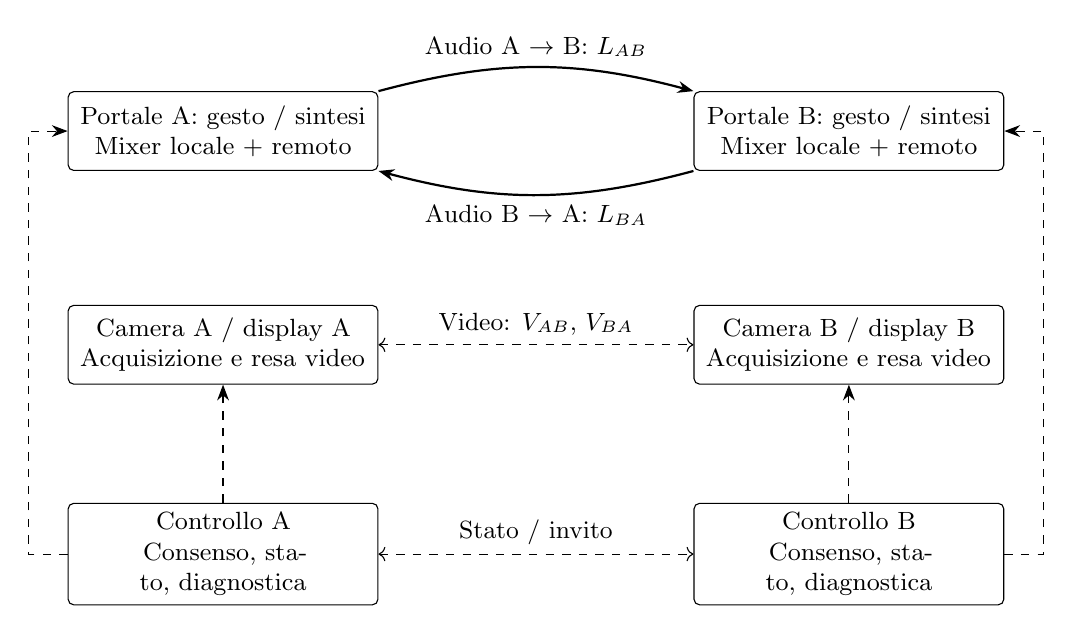
\begin{tikzpicture}[
 box/.style={draw,rounded corners=2pt,text width=3.7cm,minimum height=1cm,align=center,font=\small},
 a/.style={-{Stealth[length=2mm]},thick},
 v/.style={-{Stealth[length=2mm]},dashed}]
\node[box] (aa) {Portale A: gesto / sintesi\\Mixer locale + remoto};
\node[box,right=4cm of aa] (ba) {Portale B: gesto / sintesi\\Mixer locale + remoto};
\node[box,below=1.7cm of aa] (av) {Camera A / display A\\Acquisizione e resa video};
\node[box,below=1.7cm of ba] (bv) {Camera B / display B\\Acquisizione e resa video};
\node[box,below=1.5cm of av] (ac) {Controllo A\\Consenso, stato, diagnostica};
\node[box,below=1.5cm of bv] (bc) {Controllo B\\Consenso, stato, diagnostica};
\draw[a] (aa.north east) to[bend left=15] node[above,font=\small]{Audio A $\rightarrow$ B: $L_{AB}$} (ba.north west);
\draw[a] (ba.south west) to[bend left=15] node[below,font=\small]{Audio B $\rightarrow$ A: $L_{BA}$} (aa.south east);
\draw[v,<->] (av) -- node[above,font=\small]{Video: $V_{AB}$, $V_{BA}$} (bv);
\draw[v,<->] (ac) -- node[above,font=\small]{Stato / invito} (bc);
\draw[v] (ac.west) -- ++(-0.5,0) |- (aa.west);
\draw[v] (bc.east) -- ++(0.5,0) |- (ba.east);
\draw[v] (ac) -- (av);
\draw[v] (bc) -- (bv);
\end{tikzpicture}}
\caption{Architettura proposta a due estremità. Ogni blocco audio
contiene ascolto locale e ricezione remota, senza ritorno del segnale
ricevuto. Audio e video hanno latenze distinte da misurare nei due
sensi; le connessioni possono essere dirette oppure attraversare
un servizio intermedio. Il disegno non implica latenze simmetriche.}
\label{fig:engineering-architecture}
\end{figure}

\section{Trasportare il suono, oppure ricostruirlo da MIDI}

JackTrip offre un riferimento concreto: il progetto documenta
trasmissione audio bidirezionale multicanale non compressa e
implementazioni su più sistemi operativi \cite{net_jacktrip}.
È un candidato da integrare e confrontare, non una soluzione già
collaudata nel Portale. LoLa, sviluppato dal Conservatorio Tartini
con GARR, affronta congiuntamente audio e video per la performance
remota; il manuale 2.0.0 descrive hardware specifico e reti adeguate,
con requisiti elevati nella configurazione video non compressa
\cite{net_lola_manual}. Questi precedenti dimostrano l'esistenza del
campo tecnico, non la fattibilità automatica su una connessione
ordinaria o con una webcam qualsiasi.

L'audio trasmesso conserva il risultato sonoro prodotto dal pianista,
compresi timbro, dinamica ed effetti. Il MIDI trasmette invece eventi:
la postazione remota deve ricostruirne il suono con un sintetizzatore
\cite{eng_midi}. Banche timbriche diverse, curve di velocity, pedali,
polifonia e riverberi possono produrre esperienze differenti. Per una
modalità MIDI condivisa occorre dichiarare strumenti e mappature,
gestire ordinamento e perdita degli eventi, sincronizzare le scelte
ed evitare note sospese. Il minor traffico non elimina il tempo di
propagazione; una previsione di note future altererebbe ciò che
l'altro sta realmente suonando.

Si propone quindi audio come riferimento per la presenza musicale,
con MIDI opzionale per partitura, analisi del gesto e attività
concordate. Inviare entrambi non autorizza a sommare due riproduzioni
della stessa parte: si sceglie esplicitamente quale ascoltare.
Per due canali PCM a 48~kHz e 24 bit, il solo contenuto audio richiede
$48.000\times24\times2=2.304.000$ bit/s per direzione; intestazioni,
ridondanza e video si aggiungono. È un calcolo di dimensionamento,
non una misura di banda sufficiente per una buona esecuzione.

\section{Tre latenze che non vanno confuse}

La latenza \emph{locale} collega gesto e ascolto del proprio strumento.
La latenza \emph{unidirezionale}, $L_{AB}$, collega il gesto in A
all'ascolto in B; $L_{BA}$ descrive il verso opposto. Il \emph{round-trip}
misura un'andata e ritorno definiti: un ping di rete non include
necessariamente acquisizione, sintesi, mixer e trasduttori. Dimezzare
il ping non restituisce una misura del percorso musicale in un senso.

\[
L_{AB}=L_{\mathrm{ingresso},A}+L_{\mathrm{invio},A}
+L_{\mathrm{rete},AB}+L_{\mathrm{buffer},B}
+L_{\mathrm{uscita},B}.
\]

Le voci devono avere confini non sovrapposti; una sintesi software
può sostituire l'acquisizione analogica. Il budget locale proposto
resta mediana entro 15~ms e percentile 95 entro 20~ms, da collaudare.
Questi valori non si trasferiscono al collegamento geografico.
A 48~kHz, 128 campioni occupano 2,67~ms: moltiplicare buffer,
aggiungere codifica e attraversare la rete accumula ulteriore ritardo.

Diecimila chilometri richiedono una formulazione precisa. Usando
come esempio l'indice di gruppo $n_g=1,4682$ riportato da Corning
per una fibra convenzionale a 1550~nm \cite{net_fiber}, la sola
propagazione su 10.000~km di fibra vale:
\[
t_{\mathrm{prop}}=\frac{n_g d}{c}
\simeq\frac{1,4682\times10^{7}}{299.792.458}\ \mathrm{s}
\simeq49\ \mathrm{ms}.
\]
Circa 50~ms in un senso, dunque circa 100~ms per due percorsi
analoghi, prima di apparati, code e conversioni. Il tracciato reale
può superare la distanza geografica; questa è una stima inferiore
per l'ipotesi di fibra dichiarata, non una misura di una rotta.
Un collegamento più capiente non rimuove tale contributo.

Non ne segue che ogni esperienza musicale a quella distanza sia
priva di valore. Segue che la stessa simultaneità fisica non offre
necessariamente lo stesso accoppiamento ritmico di due pianisti
nella medesima stanza. Le prove devono distinguere repertorio,
tempo, ruolo e strategia di ascolto. Non si promette una soglia
universale oltre la quale tutta la musica smette di funzionare.

\section{Jitter, perdita e ascolto senza ritorni}

La variabilità degli arrivi, o jitter, costringe a scegliere fra
attesa e rischio di interruzione. Un buffer maggiore può rendere
continuo il suono aggiungendo ritardo; JackTrip documenta questo
compromesso e distingue diversi contributi nella diagnostica
\cite{net_jacktrip_latency}. Il test deve registrare impostazioni,
ritardi e artefatti: una barra verde non basta a descrivere
l'esperienza. Perdita casuale e raffiche di pacchetti mancanti
vanno provate separatamente.

La configurazione iniziale proposta impiega Ethernet e ascolto
cablato. Ogni estremità ha una propria coda di ricezione, poiché
le condizioni possono essere asimmetriche. Eventuali tecniche di
ridondanza o ricostruzione dei campioni devono essere dichiarate:
mascherare un'interruzione non equivale a recuperare con certezza
l'esecuzione originale. Durante un cambiamento di buffer, entrambi
vedono che la modalità sonora è cambiata. Il sistema non continua
a qualificare come stabile una sessione che sta degradando.

Le cuffie semplificano la prima configurazione full duplex. Con
diffusori e microfono aperto occorre controllare rientri acustici,
eco e feedback. La cancellazione d'eco pensata per il parlato
può alterare suoni sostenuti e sovrapposti: va valutata musicalmente,
non attivata come garanzia generica. Il mixer invia soltanto fonti
locali e mantiene regolazioni indipendenti per sé, interlocutore
e voce. La perdita di un dispositivo silenzia il percorso guasto;
il ripristino non riapre automaticamente microfoni o livelli elevati.

\section{Il quasi specchio: camera, sguardo e tempo audiovisivo}

Lo schermo OLED è una scelta espressiva da verificare insieme a
luminosità, riflessi, dimensione percepita e input lag. La velocità
del pannello non equivale alla latenza camera--display. Esposizione,
acquisizione, codifica, rete, decodifica e visualizzazione possono
ritardare l'immagine. A 60 immagini al secondo un intervallo dura
16,7~ms, ma l'intera catena può richiederne diversi. LoLa è
particolarmente pertinente proprio perché considera acquisizione
e resa audiovisiva come un sistema \cite{net_lola_manual}.

La camera principale dovrebbe avvicinarsi all'asse dello sguardo;
un'inquadratura aggiuntiva delle mani può servire all'osservazione
tecnica. La scelta va prototipata con persone di stature differenti,
sedute e in piedi: guardare il volto sullo schermo non significa
guardare nella camera. L'immagine quasi speculare è un'ipotesi
percettiva, non una giustificazione per invertire automaticamente
mani e tastiera. Orientamento, scala e anteprima locale devono
restare chiari al partecipante.

Si misura separatamente lo scarto $\Delta_{AV}=V_{AB}-L_{AB}$,
riferendo entrambe le catene allo stesso evento fisico e alla stessa
origine temporale. Con riferimenti diversi la sottrazione non descrive
lo scarto percepito fra gesto e suono.
Ritardare l'audio per allinearlo a un video lento può peggiorare
l'interazione musicale. In modalità ensemble si privilegia la
catena audio e si esplicita l'eventuale scarto; in una dimostrazione
si può concordare un diverso compromesso. Nessuna correzione
può mostrare un gesto futuro: la sincronizzazione va ottenuta
riducendo ritardi o introducendo attese note, non inventando
movimenti del pianista.

\section{Pratiche connesse e piattaforma di studio}

Il Portale propone tre regimi espliciti. Nell'\emph{ensemble
connesso} entrambi suonano contemporaneamente, con attività e
condizioni tecniche annotate; la valutazione comprende stabilità
del tempo, ascolto reciproco e libertà espressiva. Nell'\emph{alternanza}
uno propone e l'altro risponde, senza far passare la conversazione
per un duetto simultaneo. Nel lavoro \emph{asincrono} una traccia
viene ripresa successivamente, con provenienza e tempo dichiarati.
Sono pratiche musicali proprie, non livelli di dignità del progetto.

La sperimentazione a grande distanza può includere parti sostenute,
entrate concordate, improvvisazioni che incorporano il ritardo,
un riferimento temporale condiviso o ruoli ritmici asimmetrici.
Queste sono ipotesi compositive da provare, non soluzioni universali.
Un metronomo sincronizzato aiuta a condividere un riferimento ma
non fa arrivare istantaneamente la risposta dell'altro. Il desiderio
di suonare insieme resta la domanda che guida il confronto.

La piattaforma di studio può essere propria oppure collegare
risorse esterne. Deve distinguere materiale curato, sessione dal
vivo e registrazione, consentire scelta di repertorio e scambio
di annotazioni, dichiarare licenze e disponibilità offline.
L'integrazione con un servizio esistente richiede verifica di
accessibilità, esportazione, costi e trattamento dei dati. Non è
necessario costruire un nuovo sistema di videoconferenza per
rendere originale l'esperienza del Portale.

Un aiuto AI può spiegare o proporre un esercizio fuori dal percorso
audio in tempo reale. Non sostituisce l'interlocutore con una
simulazione non dichiarata, non attribuisce note previste al
pianista remoto e non valuta automaticamente l'apprendimento.
Risposte tardive vengono eliminate alla chiusura della sessione.

\section{Invito, consenso e guasto leggibile}

La macchina di stati proposta attraversa \emph{disponibile},
\emph{invito}, \emph{accettazione reciproca}, \emph{prova audio-video},
\emph{sessione}, \emph{degradazione}, \emph{chiusura} e \emph{ripristino}.
Prima dell'accettazione non vengono trasmessi audio o video.
La camera può essere attivata su scelta per la sola anteprima locale,
chiaramente distinta dalla trasmissione; il microfono resta chiuso
finché non viene abilitato per la prova concordata. La prova rende udibili i livelli, verifica la
presenza del partner e mostra la modalità concordata. Entrambe
le persone possono interrompere immediatamente la trasmissione.

Una perdita di rete viene annunciata: nessun filmato in loop
continua a fingere presenza. Il nucleo locale resta suonabile,
ma una ripresa del collegamento richiede conferma, evitando di
riaprire una stanza privata senza preavviso. Passare da ensemble
ad alternanza richiede una scelta condivisa; disattivare la rete
non equivale ad aver completato l'esperienza promessa.

Le sessioni non sono registrate per impostazione iniziale. Un'eventuale
registrazione o trasmissione pubblica richiede un accordo distinto,
con indicazione persistente su entrambi i lati. Inviti temporanei,
autenticazione delle estremità e protezione del trasporto devono
essere verificati nella tecnologia selezionata: un protocollo audio
veloce non offre automaticamente queste proprietà. Le porte di
amministrazione restano separate; i log tecnici escludono contenuti
musicali, immagini e conversazioni salvo ricerca specificamente
concordata.

\section{Collaudo a due estremità e decisioni di progetto}

Il banco iniziale confronta due postazioni sulla stessa rete,
poi una tratta geografica dichiarata e infine condizioni più
impegnative. Si conservano versione software, interfacce, campionamento,
buffer, codec, risoluzione video, instradamento noto e orario della
prova. Un clock condiviso sufficientemente accurato permette
misure unidirezionali; in sua assenza si dichiarano incertezza
ed eventuale sola misura di andata e ritorno. La sincronizzazione
ordinaria dell'orologio non viene presunta precisa al millisecondo.

\begin{table}[htbp]
\centering\small
\begin{tabularx}{\linewidth}{@{}lX@{}}
\toprule
Prova & Evidenza richiesta prima di dichiarare la funzione verificata \\
\midrule
N1 Locale & Gesto--suono in A e B: mediana, p95, massimo, incertezza; confronto col budget locale. \\
N2 Trasporto & $L_{AB}$ e $L_{BA}$, oppure RTT esplicitamente qualificato; non usare ping come misura completa. \\
N3 Continuità & Jitter, perdita e raffiche simulate: artefatti, cambi di buffer, tempi di recupero. \\
N4 Presenza & Camera--display e scarto audio-video nei due sensi; scala, orientamento e sguardo valutati con persone. \\
N5 Musica & Stesso compito in presenza e connesso: andamento temporale, interruzioni e giudizi dei partecipanti. \\
N6 Controllo & Invito rifiutato, revoca, rete caduta, riconnessione: nessuna ripresa non autorizzata. \\
N7 Isolamento & Arresto UI, cavo MIDI scollegato, audio perso: nessuna nota sospesa e guasto riconoscibile. \\
N8 Cura & Ripristino da configurazione versionata e prova prolungata; log privi di contenuti personali non previsti. \\
\bottomrule
\end{tabularx}
\caption{Matrice di collaudo proposta. Nessuna prova è dichiarata
eseguita sul Portale. Le condizioni musicali fanno parte del risultato.}
\end{table}

Le misure tecniche vanno accompagnate da esercizi ripetuti e
resoconti dei due pianisti, evitando di trasformare un'esecuzione
riuscita in garanzia per ogni brano. Il software deve essere
ricostruibile con licenze, dipendenze e configurazioni documentate;
la manutenzione comprende anche camera, cablaggi, ventilazione,
limiti d'ascolto e protezioni fisiche. Un secondo operatore deve
poter ricreare la sessione, non soltanto guardare un video del test.

La sfida non è far sparire la distanza con una dichiarazione.
È costruire una relazione in cui vedere, suonare e rispondere
restino leggibili alle due persone. Il Portale diventa tecnicamente
credibile quando sa mostrare le condizioni nelle quali quella
presenza riesce, e dare forma musicale anche alle distanze che
non può cancellare.

\chapter{Imparare musica, diventare risorsa per qualcuno}\label{sec:learning}

Il valore educativo del Portale comincia da una possibilità molto concreta:
una persona che non si considera musicista può produrre un suono, ascoltare
una risposta e scoprire di avere qualcosa da proporre. La città le offre
uno strumento e un interlocutore prima di chiederle un'iscrizione, un titolo
o una prestazione. Questa apertura costituisce una scelta politica del
progetto; la sua efficacia educativa resta da verificare. Un oggetto molto
frequentato potrebbe offrire soprattutto intrattenimento. Un laboratorio
musicalmente riuscito potrebbe raggiungere soltanto chi possiede già
strumenti culturali e tempo libero. La ricerca deve rendere visibili entrambe
le possibilità, senza ridurre il piacere di suonare a un punteggio.

\section{Una teoria del cambiamento esposta alla prova}

Proponiamo una catena di cinque passaggi. L'accesso gratuito e comprensibile
abbassa il costo del primo tentativo; una risposta sonora controllabile rende
leggibile il rapporto tra gesto e risultato; un compito condiviso richiede
ascolto e negoziazione; la restituzione tra partecipanti rende comunicabile
una scoperta; una risorsa riutilizzabile e un appuntamento successivo
permettono di riprenderla. Le risorse necessarie sono uno strumento affidabile,
un ambiente praticabile, tempo di facilitazione e una piccola redazione
dei materiali. Gli esiti attesi sono autonomia musicale circoscritta,
capacità di aiutare un compagno e continuità della pratica. Sono ipotesi
del progetto, non risultati già osservati.

Ogni passaggio può interrompersi. Un'interfaccia appariscente può attirare
senza risultare comprensibile; una coppia può dividersi in esecutore e
spettatore; un tutorial può sostituire l'ascolto; un esercizio salvato può
non essere più aperto. Registrare soltanto accessi o minuti di permanenza
nasconderebbe questi fallimenti. La valutazione deve seguire le transizioni:
quanti iniziano senza aiuto, quanti assumono entrambi i ruoli, che cosa
sanno rifare, che cosa riprendono in seguito. Il diritto di partecipare
rimane indipendente dall'accettazione di essere valutati.

\section{Peeragogy, corpo e attenzione condivisa}

Nel \emph{Peeragogy Handbook}, l'apprendimento e la produzione di conoscenza
tra partecipanti si organizzano attraverso obiettivi e strutture che il
gruppo può modificare \cite{learn_peeragogy}. Nel Portale questa impostazione
diventa una regola operativa: ciascuno deve poter scegliere, provare,
spiegare e correggere una parte del lavoro comune. Essere pari non significa
possedere la stessa competenza. Un pianista esperto può apprendere da chi
propone un ritmo, conosce un repertorio diverso o riconosce una difficoltà
di accesso che il pianista non incontra.

La dimensione corporea va progettata nei gesti: percepire la durata di una
pressione, anticipare un ingresso, dosare l'intensità, lasciare spazio al
suono altrui. Per il prototipo assumiamo che rendere questi rapporti
percepibili favorisca l'esplorazione intenzionale; sarà necessario
osservarlo. Lo schermo può visualizzare l'alternanza dei turni o una
struttura ritmica, ma deve poter essere oscurato. Se il partecipante segue
soltanto un indicatore luminoso e non riconosce più la frase ascoltandola,
il supporto ha prodotto dipendenza dal suggerimento. La prova senza schermo
serve precisamente a distinguere le due situazioni.

Una \emph{scoping review} di 28 studi empirici pubblicati tra il 2006 e il
2023 descrive motivazione, identità e pratiche dell'apprendimento musicale
informale \cite{weatherly2025}. Pubblicata online nel settembre 2024 e nel
fascicolo del 2025, offre una mappa, non una stima unica dell'effetto. Gli
autori discutono limiti di generalizzazione e campioni piccoli; nella
selezione sono esclusi lavori focalizzati sulla musica digitale o
sull'apprendimento virtuale. Non sostiene dunque, da sola, l'efficacia
della componente digitale proposta qui.

Anche il legame tra musica e cooperazione richiede misura. Un esperimento
con bambini di quattro anni rilevò comportamenti di aiuto successivi
all'attività musicale condivisa \cite{learn_kirschner}; un successivo
esperimento sul campo non trovò gli effetti attesi della sincronizzazione
\cite{learn_baier}. Popolazioni, compiti e contesti non coincidono con un
parco urbano intergenerazionale. Assumiamo la cooperazione come pratica
da costruire e osservare, senza promettere che suonare insieme renda
automaticamente più solidale una comunità.

\section{Tre situazioni, tre apprendimenti osservabili}

\paragraph{Una domanda di quattro suoni.}
Due persone dispongono di dodici minuti. La prima inventa una frase di
quattro suoni su cinque tasti disponibili; la seconda la riprende e cambia
un elemento scelto: conclusione, durata o intensità. Dopo tre scambi
invertono i ruoli. Il facilitatore chiede: ``Che cosa hai mantenuto e che
cosa hai cambiato?'' Il materiale iniziale contiene una dimostrazione breve
e un foglio con simboli semplici, senza richiedere lettura del pentagramma.
L'obiettivo è distinguere ripetizione e trasformazione intenzionale.
L'evidenza è una nuova risposta coerente con il vincolo, seguita da una
spiegazione verbale, gestuale o musicale. Se il compagno esegue tutto,
il compito non è completato, anche quando il risultato suona bene.

\paragraph{Tenere il tempo, lasciare entrare l'altro.}
Una coppia lavora per venti minuti su due battute: un ostinato di quattro
pulsazioni e una risposta ritmica. Può scegliere tempo e timbro, usando
una tastiera divisa o due controlli accessibili. Prima prova con un
riferimento regolare, poi lo elimina per quattro ripetizioni. Si ferma,
ascolta e decide una sola correzione. I ruoli cambiano; una registrazione
MIDI locale, soltanto se accettata, permette di confrontare gli attacchi.
L'obiettivo comprende mantenere il riferimento e recuperare dopo una
perdita del tempo. Una ripartenza negoziata vale più della prosecuzione
meccanica di un accompagnamento automatico. La misura temporale accompagna
il giudizio musicale e non penalizza variazioni espressive concordate.

\paragraph{Una cartolina sonora che un'altra persona può suonare.}
In quaranta minuti, tre o quattro partecipanti compongono un frammento
originale di otto battute ispirato a un'esperienza del luogo. La relazione
con il parco può essere una pausa, un'andatura o un racconto: non occorre
registrare passanti o suoni ambientali. Il gruppo sceglie struttura,
contrasti e conclusione, prepara un audio dimostrativo e istruzioni
accessibili. Un secondo gruppo prova il materiale senza spiegazioni
aggiuntive degli autori e segnala dove si perde. La revisione di quelle
istruzioni costituisce parte del lavoro musicale. L'esito è un contributo
trasmissibile, con provenienza e condizioni di riuso controllate; il
consenso alla pubblicazione viene chiesto separatamente dalla partecipazione.

\section{Il lavoro del facilitatore e l'accesso reale}

Il facilitatore prepara materiali con difficoltà graduata, esplicita i
turni, osserva chi non riesce a entrare e interviene prima che l'abilità di
uno diventi il silenzio degli altri. Durante il compito propone una domanda
o una dimostrazione breve; poi restituisce il controllo. Nella scheda di
sessione annota numero e tipo degli aiuti, perché un risultato ottenuto
con cinque interventi non equivale allo stesso risultato autonomo. La
formazione comprende gestione degli errori, ascolto, adattamento dei
controlli e procedure di interruzione. Non basta saper suonare.

Prevediamo una modalità senza testo esteso, istruzioni ascoltabili,
dimostrazioni visive prive di lampeggiamenti, controlli adatti a una sola
mano, volume regolabile e tempi non competitivi. Questi sono requisiti da
provare con persone interessate, non una certificazione di accessibilità.
Ogni adattamento va descritto insieme al compito: una misura basata sulla
velocità delle dita non rappresenta la comprensione di chi usa un
controllo alternativo. Per le attività valutate si concorda una modalità
equivalente rispetto all'obiettivo; quando l'equivalenza non è sostenibile,
si descrive il caso senza confrontare punteggi impropriamente.

L'osservazione pubblica può scoraggiare più della difficoltà tecnica.
Servono prove a volume contenuto, possibilità di ascoltare prima di
esporsi e sessioni senza pubblico raccolto attorno allo strumento.
L'invito deve raggiungere anche chi non frequenta già scuole di musica.
Biblioteche e associazioni potranno aiutare a reclutare pubblici diversi,
se accetteranno di collaborare: non sono partner acquisiti. Nel primo
pilota proponiamo adulti; attività con minori richiedono un protocollo
dedicato e personale preparato, anziché un'estensione automatica dei
risultati degli adulti.

\section{Una memoria comune con diritti leggibili}

La raccomandazione UNESCO sulle OER richiede materiali in pubblico dominio
o con licenze che permettano accesso, riuso, adattamento e redistribuzione
\cite{unesco_oer2019}. Proponiamo per le nuove schede originali CC BY 4.0,
che consente anche adattamenti con attribuzione e indicazione delle
modifiche \cite{learn_ccby}. La concessione è irrevocabile per chi rispetta le condizioni: ritirare
un file dal catalogo non cancella i riusi già autorizzati.
È una proposta editoriale: la licenza non
viene applicata automaticamente a contributi di terzi o alle persone
registrate. Un brano reperibile online non diventa riutilizzabile perché
serve a insegnare musica.

Ogni risorsa avrà identificatore, autore o pseudonimo concordato, data,
obiettivo, prerequisiti, durata, versione, formato modificabile, licenza
e fonti degli eventuali materiali incorporati. Il curatore verifica diritti
e comprensibilità prima della pubblicazione. Se manca una base chiara per
il riuso, il contributo resta fuori dall'archivio pubblico. Si distingue
la composizione dall'esecuzione registrata e dalle istruzioni. Una
raccolta iniziale di sei schede revisionate è preferibile a un flusso
indiscriminato: permette di misurare manutenzione, riusi e correzioni.
L'accesso offline conserva utilità anche senza account o telefono.

\section{Pilota di fattibilità e apprendimento trasferibile}

Dentro la finestra di dodici settimane dello scenario economico A,
proponiamo una raccolta educativa di sei settimane, con 36 adulti organizzati in 18 coppie,
reclutati dichiarando esperienza musicale e disponibilità al richiamo.
Sono dimensioni di fattibilità dettate da tempo e presidio, non derivate
da un calcolo di potenza. Prima del reclutamento si pubblicano protocollo,
rubrica, criteri di esclusione e analisi prevista. Le prove di comprensibilità precedono l’assegnazione e non entrano nel
confronto fra condizioni; il loro numero e i cambiamenti conseguenti
vengono registrati separatamente. Le sessioni valutate mantengono
stabili esercizi e versione del software, annotando ogni modifica urgente.
Una sessione dura circa trenta minuti; il richiamo, dopo 7--14 giorni,
richiede dieci minuti.

Le coppie vengono assegnate casualmente a due condizioni, bilanciando per
quanto possibile l'esperienza iniziale: esplorazione con istruzioni di base
oppure compito strutturato con alternanza e restituzione tra pari.
Entrambe hanno uguali durata, strumento e disponibilità di assistenza
tecnica. L'unità assegnata è la coppia; trattare le 36 persone come
osservazioni indipendenti gonfierebbe l'informazione. Il confronto stima
esplorativamente il valore del pacchetto di facilitazione, non l'effetto
puro di una singola componente né il vantaggio del Portale rispetto a
una tastiera più semplice. Quest’ultimo confronto, necessario prima di
giustificare l’integrazione definitiva, richiede una fase distinta con
stessi compiti e stessa dose di facilitazione nelle due configurazioni. Lo stesso facilitatore opera in entrambe
le condizioni con un copione e tempi registrati. Soltanto dopo il richiamo differito, tutti
possono provare la modalità strutturata, evitando di alterare il confronto
prima della misura di mantenimento. La pratica svolta altrove fra le
visite viene registrata come possibile fonte di contaminazione.

Prima e dopo si richiede una breve frase ritmica; al richiamo si propone
un materiale equivalente ma nuovo. Le prove avvengono senza AI,
accompagnamento automatico, suggerimenti luminosi o aiuto del compagno.
L'AI resta esclusa da questa prima fase per rendere interpretabile il
contributo della struttura sociale. In un'eventuale fase successiva si
potrà confrontare un supporto AI specifico mantenendo queste prove autonome.
Il trasferimento riguarda un compito musicale vicino a quello esercitato;
non autorizza deduzioni su intelligenza, rendimento scolastico o benessere.

\paragraph{Misure e qualità del giudizio.}
Per il ritmo si riporta l'errore assoluto mediano degli attacchi rispetto
al riferimento, normalizzato per la durata della pulsazione, usando un
allineamento dichiarato e annotando note mancanti o aggiunte. La precisione
da sola non misura musicalità. Una rubrica a tre dimensioni valuta
riconoscibilità della frase, trasformazione intenzionale e recupero dopo
interruzione, ciascuna da 0 a 2: assente, parziale, autonomo. Due valutatori
indipendenti, senza conoscere condizione e momento della prova quando
possibile, giudicano i file codificati; si pubblicano accordo esatto,
divergenze e decisioni, prima di qualunque media aggregata.

La componente tra pari si osserva attraverso alternanza effettiva,
richieste di chiarimento e correzioni accolte: descrizioni con esempi,
senza trasformarle in una scala psicologica non validata. Si riportano
anche abbandoni, aiuti, accessi impediti, richiami mancanti e motivi
volontariamente forniti. I risultati comprendono distribuzioni e
incertezza, non soltanto una percentuale migliorata. Novità dell'oggetto,
autoselezione, pratica tra le visite e differenze tra coppie limitano
l'inferenza; un confronto piccolo non dimostra efficacia cittadina.

\paragraph{Regole per proseguire, correggere o fermarsi.}
Le seguenti soglie sono proposte gestionali da concordare prima del
pilota. Interrompere immediatamente una sessione in caso di disagio
espresso, problema di sicurezza o acquisizione di dati non prevista.
Sospendere il protocollo interessato fino alla correzione se un incidente
si ripete o emerge un ostacolo che esclude sistematicamente un pubblico.
Rivedere reclutamento e richiamo se torna meno del 60\% degli iscritti;
non dichiarare allora la ritenzione dell'apprendimento dell'intero gruppo.
Rivedere la rubrica se l'accordo esatto dei valutatori è inferiore al
75\% delle valutazioni dimensionali. Sono segnali di revisione, non soglie
scientifiche universali. Un'estensione richiede fattibilità documentata,
accesso migliorabile e risultati interpretabili; l'assenza di un vantaggio
misurato va pubblicata insieme alle esperienze riuscite.

\chapter{La città come parte dello strumento}\label{sec:city}

Una città può ospitare un'altra città nello spazio di un incontro musicale.
Una persona si siede al Portale di Bergamo e, davanti a sé, incontra un'altra
persona seduta a un secondo Portale. Lo schermo OLED e la videocamera
cercano una presenza quasi speculare: riconoscere il volto, vedere le mani,
intuire un'esitazione, cominciare insieme. La disposizione e la scala
visiva devono essere provate; la reciprocità è già un criterio del progetto.
Entrambe le persone devono poter vedere, ascoltare, proporre e interrompere.

Il nucleo dell'esperienza è suonare contemporaneamente attraverso due
luoghi. La connessione rende percepibile una distanza che per un momento
si può attraversare con un gesto musicale. La qualità tecnica del percorso
fra i due nodi decide quali gesti e repertori possono realmente convivere:
la misura della rete deve precedere la promessa pubblica del concerto.
Quando quella qualità non basta, una conversazione o uno scambio a turni
possono conservare valore, ma vanno annunciati come modalità diverse.

La bellezza civica di questa proposta risiede nella simmetria dell'invito.
Il partner remoto non fornisce un contenuto da consumare: ospita persone
che hanno a loro volta una città, un luogo e un pubblico. Curare questo
incontro significa dare a entrambi i lati tempo e iniziativa. Il Portale
può diventare una piccola infrastruttura di ospitalità reciproca, nella
quale la musica precede talvolta le parole e aiuta a trovarle.

\section{Caprotti: una scelta da argomentare}
Parco Caprotti appartiene alla geografia del documento originale del 2016;
il Padiglione del Tè è invece una candidatura sviluppata successivamente.
Questa distinzione impedisce di attribuire alla fonte un progetto localizzato
che essa non documenta. L'interesse per il Padiglione nasce dall'ipotesi
che una presenza musicale osservabile dal giardino possa costruire una
continuità fra attraversamento, curiosità e partecipazione. È un'ipotesi
spaziale da confrontare con un rilievo, con gli usi e con le condizioni reali
di accesso: trasparenza del vetro e disponibilità di uno spazio non sono
equivalenti.

Due tracce documentarie rendono più precisa la storia civica del parco.
L'inventario dell'Ufficio Tecnico registra nel 1947 una manifestazione di
volontà di donazione al Comune: documento 1435, faldone 16, pagina PDF 44.
Il documento originale non è stato consultato; l'inventario non prova
l'avvenuto trasferimento. Alla pagina PDF 65 compaiono il documento 2075,
associato a Luigi Angelini e datato 1948, e il 2076, relativo alla
Soprintendenza e datato 1950, nel faldone 30. Sono piste per una ricerca
sulle trasformazioni del giardino, non attribuzioni del progetto originario
del Padiglione \cite{mai_inventario}. La raccolta comunale IBCAA riproduce,
alla pagina PDF 176, il vincolo 118 sul Giardino Caprotti e zona di rispetto,
con decreto del 12 agosto 1949 e notifica del 10 febbraio 1950
\cite{bergamo_vincolo118}. La scheda non risolve da sola la disciplina applicabile
a un nuovo allestimento.

La verifica storica successiva dovrà ricercare progetto originario,
trasformazioni e atti relativi al manufatto. Il fascicolo di fattibilità
dovrà separatamente acquisire titolo e condizioni d'uso attuali,
competenza degli interlocutori e percorso delle eventuali autorizzazioni.
Queste due ricerche rispondono a domande diverse. Una ricostruisce ciò
che è accaduto; l'altra stabilisce ciò che possiamo proporre oggi.

\section{Un luogo già abitato da pratiche}
La pagina ufficiale del Cerchio di Gesso dedicata al \emph{Giardino
dell'anima} descrive attività di recupero e cura delle piante con volontari
e annuncia una Festa Tanabata il 7 luglio 2026 alla Sala del té di Parco
Caprotti \cite{cerchio2026}. È prova della programmazione pubblicata,
non dell'effettivo svolgimento dell'evento, della disponibilità quotidiana
della sala o dei diritti sullo spazio. È però sufficiente per richiedere
un confronto con persone e attività già presenti.

La proposta potrebbe trovare una relazione fertile con pratiche di cura:
tempi lenti, attenzione alle differenze, gesti che acquistano valore quando
vengono ripetuti insieme. Questa è una lettura progettuale, non una
collaborazione già concordata. Non autorizza a sonorizzare automaticamente
le attività esistenti. L'incontro preliminare dovrebbe produrre una mappa
condivisa degli orari, degli ingombri, dei depositi, dei momenti che
richiedono silenzio e delle attività eventualmente compatibili. Il primo
risultato utile potrebbe essere una sola giornata comune, oppure la
decisione motivata che questo luogo non sia adatto.

\section{Una coppia di luoghi, una relazione da costruire}
L'unità di progetto per gli incontri remoti è una coppia di Portali.
Un nodo può ospitare studio individuale o attività locali, ma un collegamento
civico richiede una seconda organizzazione capace di accogliere le persone,
curare il programma e garantire il presidio. Nessuna città, biblioteca,
scuola o associazione è qui indicata come partner acquisito.
La selezione dovrebbe considerare interesse reciproco, accesso pubblico,
competenze di accompagnamento, disponibilità simultanea e compatibilità
tecnica, oltre alla distanza geografica.

Si possono confrontare tre assetti: due presenze temporanee per una serie
limitata di incontri; una coppia stabile con calendario regolare; un nodo
continuativo che incontra a rotazione nodi temporanei compatibili.
Il primo assetto riduce l'impegno sul sito ma moltiplica montaggi e trasporti.
Il secondo sostiene il ritorno e le relazioni, ma richiede risorse durevoli
in entrambi i luoghi. Il terzo amplia gli interlocutori e richiede una nuova
verifica di rete, audio, immagine e gestione a ogni accoppiamento.
La compatibilità di un nodo non dimostra quella di tutte le sue connessioni.

La cura del programma può iniziare con due musicisti che si presentano
attraverso una breve frase, proseguire con variazioni condivise e aprirsi
alla partecipazione dei presenti. Musiche, età e lingue vanno scelte con
entrambi gli ospitanti. Si può lasciare a ciascuna città la proposta di una
parte degli incontri, alternando chi invita e chi risponde. Il gemellaggio
musicale è qui una possibilità progettuale, non uno status istituzionale
attribuito ai luoghi.

Fra gli appuntamenti, la modalità studio mantiene vivo il nodo: esercizi,
materiali e accompagnamento possono provenire da una piattaforma propria
o da un servizio esterno selezionato. La scelta dovrà confrontare
accessibilità, funzionamento senza account personale ove possibile,
licenze, esportazione dei materiali e dipendenza dal fornitore. Uno
strumento didattico esterno non va presentato come tecnologia originale
del Portale; la sua integrazione e la relazione con gli incontri pubblici
sono invece parte del progetto. L'eventuale piattaforma propria richiede
un budget distinto e un ambito funzionale definito.

La collocazione di ciascun nodo deve superare le verifiche su disponibilità,
accessibilità, compatibilità acustica, tutela del luogo e reversibilità.
Le evidenze mancanti restano tali: un punteggio estetico favorevole non può
compensare l'assenza di un titolo d'uso o di un percorso di accesso praticabile.

\section{Valore pubblico, attrattività e diritto di passare oltre}
L'incontro con una persona lontana può essere una porta d'ingresso, purché non diventi l'unico
criterio. Un oggetto sorprendente può generare fotografie senza produrre
scambio musicale. Il progetto dovrebbe osservare separatamente curiosità
iniziale, possibilità di cominciare, collaborazione fra persone e ritorno
nel tempo. Una visita breve può avere valore; non dimostra apprendimento.
Un numero elevato di presenze non dimostra accesso equo.

La promessa civica comprende anche chi non suona. Il giardino deve poter
continuare a ospitare riposo, conversazioni e attraversamento. Per questo
la programmazione dovrà stabilire modalità sonore, fasce temporali,
procedura di segnalazione e responsabile capace di interrompere una
sessione. Il dissenso di un residente o di un frequentatore è un dato di
progetto da esaminare, non un ostacolo comunicativo da neutralizzare.

L'accesso equo richiede scelte osservabili: ingresso gratuito alle prove
pubbliche di base; avvio senza account personale; istruzioni comprensibili;
possibilità di osservare senza partecipare; turni che non favoriscano
sempre chi ha già esperienza. Vanno provati avvicinamento, postura,
raggiungibilità dei comandi e forme alternative di interazione con persone
che presentano esigenze diverse. La gratuità non elimina barriere motorie,
sensoriali, linguistiche o sociali. Prima di parlare di accessibilità
realizzata servono prove e correzioni documentate.


La finestra verso l'altro luogo deve avere un'apertura dichiarata e una
chiusura riconoscibile. Chi attraversa il giardino non deve diventare
involontariamente comparsa di una trasmissione. Inquadratura, segnalazione
della connessione e area di partecipazione vanno progettate insieme.
La proposta assume incontri concordati e presidiati; non una finestra
permanentemente aperta sui frequentatori. Il pubblico deve sapere se vede
una persona in diretta, un materiale registrato o una schermata di studio.

\chapter{Costruire e mantenere una coppia di Portali}\label{sec:delivery}

Un incontro fra città richiede che due luoghi mantengano la stessa promessa
nello stesso momento. Quando il collegamento si apre, entrambi devono
avere una persona presente, uno strumento funzionante e qualcuno capace
di accogliere il pubblico. La continuità del servizio è quindi una proprietà
della coppia: un nodo disponibile non basta a garantire l'incontro.
I ruoli e gli accordi qui descritti sono proposte, non incarichi assegnati.

\section{Governare l'incontro da entrambi i lati}
Il responsabile comune del programma concorda obiettivi, calendario,
budget e versione tecnica con un referente per ciascun luogo.
Ogni ospitante risponde di disponibilità, accesso, custodia e convivenza
con le altre attività del proprio sito. Il coordinatore tecnico della
coppia tiene la matrice di compatibilità, le misure e le procedure di
ripristino; un referente locale per nodo segue installazione e guasti.
Il coordinatore educativo concorda le attività con i facilitatori.
La gestione dei dati deve avere responsabilità dichiarate fra i soggetti
coinvolti e procedure definite prima della raccolta.

Il calendario riporta entrambi gli orari locali, i fusi e una data comune
non ambigua; considera cambi d'ora e disponibilità reali delle persone.
La finestra di preparazione deve consentire una prova fra i due facilitatori
prima dell'apertura pubblica. Assenza di un facilitatore, mancata risposta
del partner o anomalia tecnica fanno scattare la procedura concordata:
rinvio, annullamento o passaggio esplicito alla modalità studio locale.
Un'ora di attesa davanti a uno schermo vuoto sarebbe un fallimento di
ospitalità prima ancora che di tecnologia.

Ciascun partecipante può chiedere di interrompere la propria partecipazione;
ciascun facilitatore deve poter chiudere immediatamente il collegamento dal
proprio nodo. La chiusura deve essere segnalata anche all'altro lato, senza
richiedere un suo assenso per fermare audio e immagine locali. Si definiscono
in anticipo condotte ammesse, gestione dei comportamenti inappropriati,
contatto per reclami e procedura per incidenti. Gli aspetti autorizzativi,
assicurativi e di utilizzo dei contenuti musicali richiedono verifiche
specifiche: la pubblicazione non attribuisce diritti sui brani eseguiti.

La configurazione proposta non registra ordinariamente audio e video.
Qualsiasi registrazione o raccolta educativa aggiuntiva richiede finalità,
procedura e condizioni proprie, distinte dalla semplice partecipazione.
Prima dell'uso si verificano anche i comportamenti effettivi delle
piattaforme esterne: impostare il nodo senza registrazione non dimostra
che un servizio remoto non conservi dati. Inquadrature circoscritte,
stato della connessione visibile e schermata neutra a sessione chiusa
sono requisiti operativi della relazione fra i luoghi.

\section{Tre fasi di sviluppo tecnico, senza scorciatoie geografiche}
\begin{description}
\item[Fase 1: due nodi in condizioni locali controllate.]
Si costruisce la coppia e si verifica l'intera catena: strumenti, audio,
OLED, videocamere, elaborazione e collegamento. Si provano orientamento
quasi speculare, comprensibilità dei gesti, avvio reciproco e arresto.
La prova comprende ripristino e sostituzione di componenti. Il suo risultato
caratterizza quella configurazione; non dimostra ancora un servizio fra città.
\item[Fase 2: collegamento regionale.]
Due luoghi disponibili vengono collegati e misurati nelle fasce previste
per l'uso pubblico. La distanza regionale è un criterio di progressione
organizzativa, non una garanzia di bassa latenza: conta il percorso reale
dei segnali. Le prove musicali stabiliscono quali attività simultanee sono
sostenibili con quella coppia e quali condizioni richiedono sospensione.
\item[Fase 3: lunga distanza da caratterizzare.]
Si studia un ulteriore collegamento dopo le verifiche precedenti,
considerando percorso di rete, sincronizzazione audiovisiva, variabilità,
fusi orari e organizzazione. Non si promette anticipatamente esecuzione
simultanea fluida a qualunque distanza. Le attività alternative si
presentano con il loro nome; non sostituiscono silenziosamente la prova
della prestazione musicale richiesta.
\end{description}

I criteri tecnici del capitolo dedicato all'architettura devono diventare
un verbale per ciascuna coppia: configurazione, luogo, orario, misure,
attività provate, esiti e limiti. Un cambio di connessione, software o
periferica che interessa il percorso critico richiede una verifica mirata.
Per la modalità studio si prova separatamente la disponibilità dei
materiali e il funzionamento della piattaforma scelta, propria o esterna.

\section{Dodici settimane di programma pubblico}
Il pilota proposto comprende dodici settimane, con due appuntamenti
connessi settimanali di due ore. Sono 24 incontri e 48 ore di servizio
congiunto; ciascun nodo ospita le stesse 48 ore. La somma delle ore nei
due luoghi è 96, ma non va presentata come 96 ore distinte di collegamento.
Si aggiunge, per ogni appuntamento e per ogni facilitatore, un'ora di
preparazione e chiusura. Servono quindi 144 ore complessive di facilitazione,
72 per nodo. Trasporti straordinari e formazione iniziale vanno conteggiati
separatamente quando necessari.

Il programma segue le verifiche tecniche e non include automaticamente
le tre fasi geografiche. La ricerca educativa riguarda un sottoinsieme
consenziente e predefinito, con propri criteri e calendario. Incontri,
persone, sessioni di studio e ore di collegamento restano conteggi distinti.

\section{Costi comuni e costi per nodo}
Le seguenti sono \textbf{stime illustrative di pianificazione}, non
preventivi, prezzi verificati sul mercato o finanziamenti disponibili.
Si assumono 55 euro per ora tecnica e 35 euro per ora di facilitazione,
unicamente per rendere riproducibile il calcolo. Imposte, forma contrattuale
e oneri effettivi devono essere definiti nella preventivazione. Le dotazioni
sono accantonamenti per strumenti, OLED, videocamera, audio, calcolo e
involucro: una distinta componenti dovrà sostituirli prima dell'acquisto.

\begin{description}
\item[A --- Coppia per il pilota di dodici settimane.]
Sviluppo comune e documentazione: 240 ore tecniche, 13200 euro.
Dotazione: $2\times6000=12000$ euro. Messa in servizio locale:
$2\times24\times55=2640$ euro. Investimento iniziale: 27840 euro.
L'esercizio comprende 144 ore di facilitazione, 5040 euro;
assistenza comune di 24 ore, 1320 euro; assistenza locale di 12 ore
per nodo, 1320 euro complessivi; logistica e consumabili, 600 euro
per nodo, 1200 euro; servizi condivisi, 600 euro.
Esercizio: 9480 euro. Subtotale: 37320 euro; con riserva del 20\%:
\textbf{44784 euro}.
\item[B --- Coppia per un programma annuale regolare.]
Sviluppo comune: 400 ore tecniche, 22000 euro. Dotazione:
$2\times9000=18000$ euro. Messa in servizio:
$2\times48\times55=5280$ euro. Investimento iniziale: 45280 euro.
Si ipotizzano 36 settimane e due incontri settimanali: 72 incontri,
144 ore di collegamento e 432 ore complessive di facilitazione,
15120 euro. Assistenza comune: 72 ore, 3960 euro; assistenza locale:
36 ore per nodo, 3960 euro complessivi; logistica e consumabili:
1200 euro per nodo, 2400 euro; servizi condivisi: 1200 euro.
Esercizio: 26640 euro. Subtotale del primo anno: 71920 euro;
con riserva del 20\%: \textbf{86304 euro}.
\end{description}

A e B sono scenari alternativi calcolati da zero, non costi cumulativi.
Il passaggio da A a B richiederebbe un computo delle componenti riutilizzabili,
non la somma dei due totali. La fase di lunga distanza non ha qui un prezzo:
richiede un preventivo successivo alla caratterizzazione della connessione.
Una seconda persona di presidio in ciascun nodo raddoppierebbe la sola
voce di facilitazione, non lo sviluppo comune né tutto il budget.

Sono esclusi opere e adeguamenti dei siti, canoni, connettività dedicata,
trasferte straordinarie, ricerca scientifica indipendente, verifiche
specialistiche, permessi, assicurazioni e licenze musicali o didattiche.
Le ore comuni coprono l'integrazione di una configurazione circoscritta;
non stimano una piattaforma educativa proprietaria completa o l'addestramento
di modelli di intelligenza artificiale. Queste voci devono essere
quantificate prima del budget esecutivo. La riserva non le rende incluse.

Il costo totale di possesso deve distinguere parte comune e due nodi:
\[
\mathrm{TCO}_{N}=C_{\mathrm{comune},0}
+\sum_{i=1}^{2} C_{i,0}
+\sum_{t=1}^{N}\left(O_{\mathrm{comune},t}
+\sum_{i=1}^{2}O_{i,t}\right)
+C_{\mathrm{uscita}}-V_{\mathrm{residuo}}.
\]
Gli $O$ comprendono personale, manutenzione, servizi, sostituzioni e oneri
realmente applicabili. Per B, a costi invariati, le sole voci stimate danno
$45280+3\times26640=125200$ euro su tre anni, oppure 150240 euro con
la riserva proposta: un subtotale, non il TCO completo. Il modello
preliminare non applica attualizzazione. Ore volontarie e beni prestati
vanno esposti separatamente: riducono l'esborso, non il lavoro necessario.

\section{Manutenzione, passaggi decisionali e arresto}
Ogni apertura richiede controllo locale e prova fra i nodi. Configurazioni
e ripristino devono essere utilizzabili anche da un secondo operatore.
Gli aggiornamenti sono collaudati sulla coppia; il registro dei guasti
indica nodo, sintomo, intervento ed esito.

\begin{description}
\item[G0: disponibilità della coppia.]
Interlocutori legittimati, condizioni d'uso e risorse iniziali per entrambi
i luoghi. Si cambia sito se un nodo non può rispettare accesso o convivenza.
\item[G1: due nodi controllati.]
Prove della fase locale e criticità di sicurezza risolte prima dell'apertura.
\item[G2: connessione qualificata.]
Prova nel percorso reale, attività musicali validate per quella configurazione,
comandi di interruzione efficaci e responsabilità operative concordate.
\item[G3: programma pubblico.]
Calendario, personale e risorse coperti nei due luoghi. Assenza di presidio,
problemi di sicurezza o perdita delle condizioni necessarie all'attività
sospendono il collegamento; la modalità studio resta disponibile soltanto
se verificata e chiaramente annunciata.
\item[G4: continuità o conclusione.]
Esiti, accessibilità, costi e qualità dell'incontro orientano prosecuzione,
modifica o conclusione. Ritiro dei nodi, riuso e cancellazione dei dati
vanno concordati prima dell'apertura.
\end{description}


\chapter{Imparare alla presenza di qualcuno}\label{ch:synthesis}

Il Portale prende il proprio nome sul serio quando il vetro smette di essere soltanto una superficie per contenuti e diventa il luogo in cui un'altra persona può apparire, ascoltare e rispondere. La scoperta non consiste nel dimenticare che ci separa una tecnologia. Consiste nell'accorgersi che, attraverso quella tecnologia, possiamo fare qualcosa insieme che prima richiedeva di essere nello stesso luogo.

L'immagine quasi speculare dà una forma a questa possibilità. Due persone occupano posizioni corrispondenti senza diventare uguali. Una conosce un passaggio, l'altra propone un ritmo; una mostra, l'altra trova un modo diverso di eseguirlo. La musica permette alla conoscenza di passare attraverso il gesto, l'ascolto, la ripetizione e la variazione. La piattaforma di studio conserva materiali e percorsi; l'incontro li rimette in movimento.

\section{Le decisioni che seguono da questa idea}
La coppia di postazioni è l'unità minima per valutare la promessa relazionale. Il collaudo di una sola non basta. Volto e mani devono essere leggibili e l'audio deve permettere di distinguere il proprio gesto da quello remoto. Il collegamento deve essere reciproco e riconoscibile, con la libertà di chiudere camera, microfono e sessione. Una registrazione disponibile per lo studio va dichiarata come registrazione: non può occupare furtivamente il posto di una persona.

La musica simultanea richiede una verifica specifica della tratta e dell'attività. La distanza non viene cancellata da una scelta grafica o da un algoritmo di predizione. Può però essere compresa, misurata e abitata attraverso diverse pratiche musicali. Un sistema che rende esplicite le proprie condizioni permette ai partecipanti di scegliere; uno che promette assenza di ritardo e restituisce un'esperienza incoerente consuma la fiducia su cui l'incontro si regge.

Lo studio individuale è una funzione piena. Deve poter cominciare senza un interlocutore disponibile e mantenere continuità con gli incontri: una frase da riprendere, una difficoltà da esplorare, una composizione da offrire alla visita successiva. Una piattaforma propria ha senso se rende questi passaggi più semplici; le risorse esterne hanno valore quando sono accessibili, pertinenti e utilizzabili nelle condizioni reali del luogo. L'AI resta un supporto eventuale e distinto dalla presenza umana.

La città entra nella relazione con i propri tempi e responsabilità. Occorrono orari compatibili, persone che preparino l'incontro, cura dello strumento e attenzione a chi attraversa il giardino senza voler partecipare. Collegare due città richiede che entrambe possano dare e ricevere: repertori, domande, scoperte e tempo. Una rete cresce bene se ciascun luogo può riconoscersi nel progetto comune.

\section{Che cosa dobbiamo poter apprendere dalla prima prova}
La prima coppia funzionante deve permettere di osservare se la presenza dell'altro è comprensibile e desiderabile; se la persona riesce a orientare camera, ascolto e attività senza perdersi nell'interfaccia; quali pratiche musicali sopportano le condizioni della tratta; che cosa resta appreso quando il partner e i suggerimenti non ci sono più. Queste domande richiedono misure diverse. Sentirsi vicini non equivale a tenere lo stesso tempo; tenere il tempo non dimostra automaticamente un apprendimento duraturo.

Un risultato può suggerire un cambio d'inquadratura, un altro percorso di rete, una diversa attività, più facilitazione o un ambiente di studio più semplice. Può anche mostrare che una normale configurazione di videolezione offre risultati equivalenti a minor costo. Il Portale deve rendere discutibile il proprio valore aggiunto: la forma, il rapporto con lo spazio pubblico e la continuità fra studio e incontro devono giustificare il lavoro necessario a realizzarli.

\section{Una forma di vicinanza da costruire}
Vorrei conservare, alla fine del progetto tecnico, la scena che lo ha generato: qualcuno alza gli occhi dalla tastiera e trova una persona che lo sta ascoltando. Non sa ancora che cosa suoneranno, né se riusciranno subito a capirsi. Sa che dall'altra parte c'è spazio per una risposta.

Il carattere poetico del Portale vive in questa apertura. Una città può offrirla a chi non dispone di uno strumento, di un insegnante vicino o di un compagno con cui provare. Può anche offrirla a un musicista esperto che desideri incontrare un altro modo di ascoltare. La tecnologia aumenta la portata dell'incontro; l'apprendimento cresce nella qualità dell'attenzione che le persone riescono a dedicarsi.

Questa è la promessa che vale la pena costruire con precisione: dare un luogo a una vicinanza possibile, lasciando che la musica attraversi la distanza e che ciascuno possa tornare al proprio studio con qualcosa ricevuto da un altro.

\appendix
\chapter{Requisiti trasversali e percorso di verifica}\label{app:requirements}

La matrice rende rintracciabile il passaggio dalla promessa alla prova. Gli identificatori R01--R12 sono requisiti trasversali di questa edizione, non certificazioni. Le soglie quantitative dei capitoli specialistici restano candidate: prima della sperimentazione il gruppo di progetto deve congelare configurazione, procedure, denominatori e responsabilità in una scheda di collaudo versionata.

\small
\begin{longtable}{P{0.07\linewidth}P{0.25\linewidth}P{0.29\linewidth}P{0.27\linewidth}}
\toprule
ID & Requisito proposto & Prova e traccia richiesta & Condizione di decisione \\\midrule
\endfirsthead
\toprule ID & Requisito proposto & Prova e traccia richiesta & Condizione di decisione \\\midrule
\endhead
R01 & Il primo suono non richiede account, rete o AI. & Avvio da macchina spenta con rete scollegata; percorso osservato e log locale tecnico. & Bloccare apertura se il nucleo musicale dipende da autenticazione o rete. \\\addlinespace
R02 & Il gesto conserva una risposta musicale controllabile. & Misura end-to-end con catena e carico dichiarati; distribuzione di latenza e prove di note bloccate. & Confrontare soglie del capitolo tecnico; correggere prima di esporre al pubblico. \\\addlinespace
R03 & Una persona può uscire senza lasciare contenuti alla successiva. & Uscita volontaria, timeout, crash e riavvio; controllo di memoria e archivi. & Nessun contenuto di sessione deve ricomparire; conservazione solo per percorso esplicito. \\\addlinespace
R04 & L'ascolto condiviso è una scelta reversibile. & Verifica di avvio silenzioso, passaggio cuffia/diffusione e controllo livello; osservazione sul sito. & Sospendere diffusione se compromette altri usi o non rispetta condizioni concordate. \\\addlinespace
R05 & Due partecipanti possono contribuire e scambiarsi ruolo. & Attività a coppie; codifica di contributi, turni, aiuti e posizione fisica. & Rivedere spazio o attività se il secondo rimane sistematicamente spettatore. \\\addlinespace
R06 & Accessibilità verificata sull'intera catena d'uso. & Arrivo, avvicinamento, postura, comando, feedback e uscita con utenti dalle esigenze diverse. & Un'interfaccia accessibile non compensa un percorso o una struttura inaccessibili. \\\addlinespace
R07 & Il materiale distingue autore, licenza e provenienza. & Audit del pacchetto offline e dei contributi pubblicati; scheda per ciascuna risorsa. & Non pubblicare contenuti senza diritto e condizioni di riuso verificati. \\\addlinespace
R08 & L'effetto educativo è distinto dall'attrazione. & Compito musicale iniziale, successivo e differito senza supporto; abbandoni e aiuti registrati. & Non affermare apprendimento sulla sola permanenza o soddisfazione. \\\addlinespace
R09 & La collocazione è consentita e compatibile. & Sopralluogo, disponibilità documentata, verifica degli usi e dei passaggi autorizzativi. & Nessuna installazione pubblica sulla sola base del render o della proposta editoriale. \\\addlinespace
R10 & Ogni ora di apertura ha una responsabilità operativa. & Calendario, referente, procedura guasti, disponibilità dei ricambi e risorse impegnate. & Ridurre apertura se manca copertura effettiva; dichiarare servizio assistito. \\\addlinespace
R11 & Il costo include cura e continuità. & Distinta, preventivi, ore, sostituzioni e scenari di utilizzo; confronto alternativa semplice. & Ridimensionare se il costo sostenibile dipende da lavoro non riconosciuto. \\\addlinespace
R12 & Il valore aggiunto è confrontabile. & Protocollo uguale per alternativa semplice e Portale, con dose di facilitazione dichiarata. & Separare beneficio del programma, del facilitatore e della specifica tecnologia. \\
\bottomrule
\end{longtable}
\normalsize

\section{Dati mancanti che cambiano una decisione}
I dati da ottenere per primi sono quelli capaci di cambiare la configurazione: geometria e accessi reali del sito; disponibilità e usi concordabili; condizioni elettriche e ambientali; possibilità di ascolto; bisogni dei partecipanti; persone e risorse per il presidio. La raccolta di questi elementi precede un disegno costruttivo definitivo. La provenienza deve accompagnare ciascun parametro: misura diretta, documento, stima, convenzione o ipotesi.

La storiografia mantiene una propria agenda: documenti edilizi del Padiglione, attribuzione, trasformazioni, atti relativi al passaggio del giardino e quadro specifico della tutela. La data 1890 riportata nel resoconto locale \cite{primabergamo2024}
contrasta con il 1891 registrato nella fonte PUB-S07 del dossier:
la datazione resta aperta e non viene risolta per maggioranza delle fonti. Le fonti archivistiche localizzate nell'inventario non devono essere trattate come atti integralmente consultati.

\section{Materiali per una revisione riproducibile}
Il repository contiene sorgente LaTeX, bibliografia, illustrazione originale con provenienza, note di ricerca per ciascun ambito e protocollo comparativo. La valutazione va riferita a un commit preciso: il ramo principale può cambiare. Il revisore deve indicare pagine, requisiti e fonti a sostegno di ogni punteggio; i criteri che non può valutare vanno marcati come tali.

Il confronto con un altro LLM è predisposto come procedura, non presentato come risultato. Richiede un brief comune, un corpus congelato, condizioni di ricerca dichiarate, output indipendenti e valutatori che non conoscano, ove possibile, l'autore della redazione. Una buona compilazione dimostra integrità editoriale, non superiorità scientifica o fattibilità fisica. La griglia completa e il prompt per il concorrente sono nella cartella \texttt{review/}.

\bibliographystyle{plainnat}
\bibliography{references}
\end{document}
